\section*{Часто используемые ядра \(K(r)\)}

\begin{figure}[ht]
    \centering
    \includegraphics[width=\textwidth]{chapters/metric/images/I1.png}
    \caption{Графики ядер}
    \label{fig:kernels}
\end{figure}

\begin{align*}
\Pi(r) &= [{\lvert r \rvert \leq 1}] \quad \text{— прямоугольное} \\
T(r) &= (1 - \lvert r \rvert) [{\lvert r \rvert \leq 1}] \quad \text{— треугольное} \\
E(r) &= (1 - r^2) [{\lvert r \rvert \leq 1}] \quad \text{— квадратичное (Епанечникова)} \\
Q(r) &= (1 - r^2)^2 [{\lvert r \rvert \leq 1}] \quad \text{— квартическое} \\
G(r) &= \exp(-2r^2) \quad \text{— гауссовское}
\end{align*}


\section*{Выбор ядра \(K\) и ширины окна \(h\)}

\noindent
\(h \in \{\textcolor{red}{0.1}, 1.0, \textcolor{blue}{3.0}\}\), гауссовское ядро \(K(r) = \exp(-2r^2)\).
Графики с различной шириной окна \(h\):
\begin{figure}[ht]
    \centering
    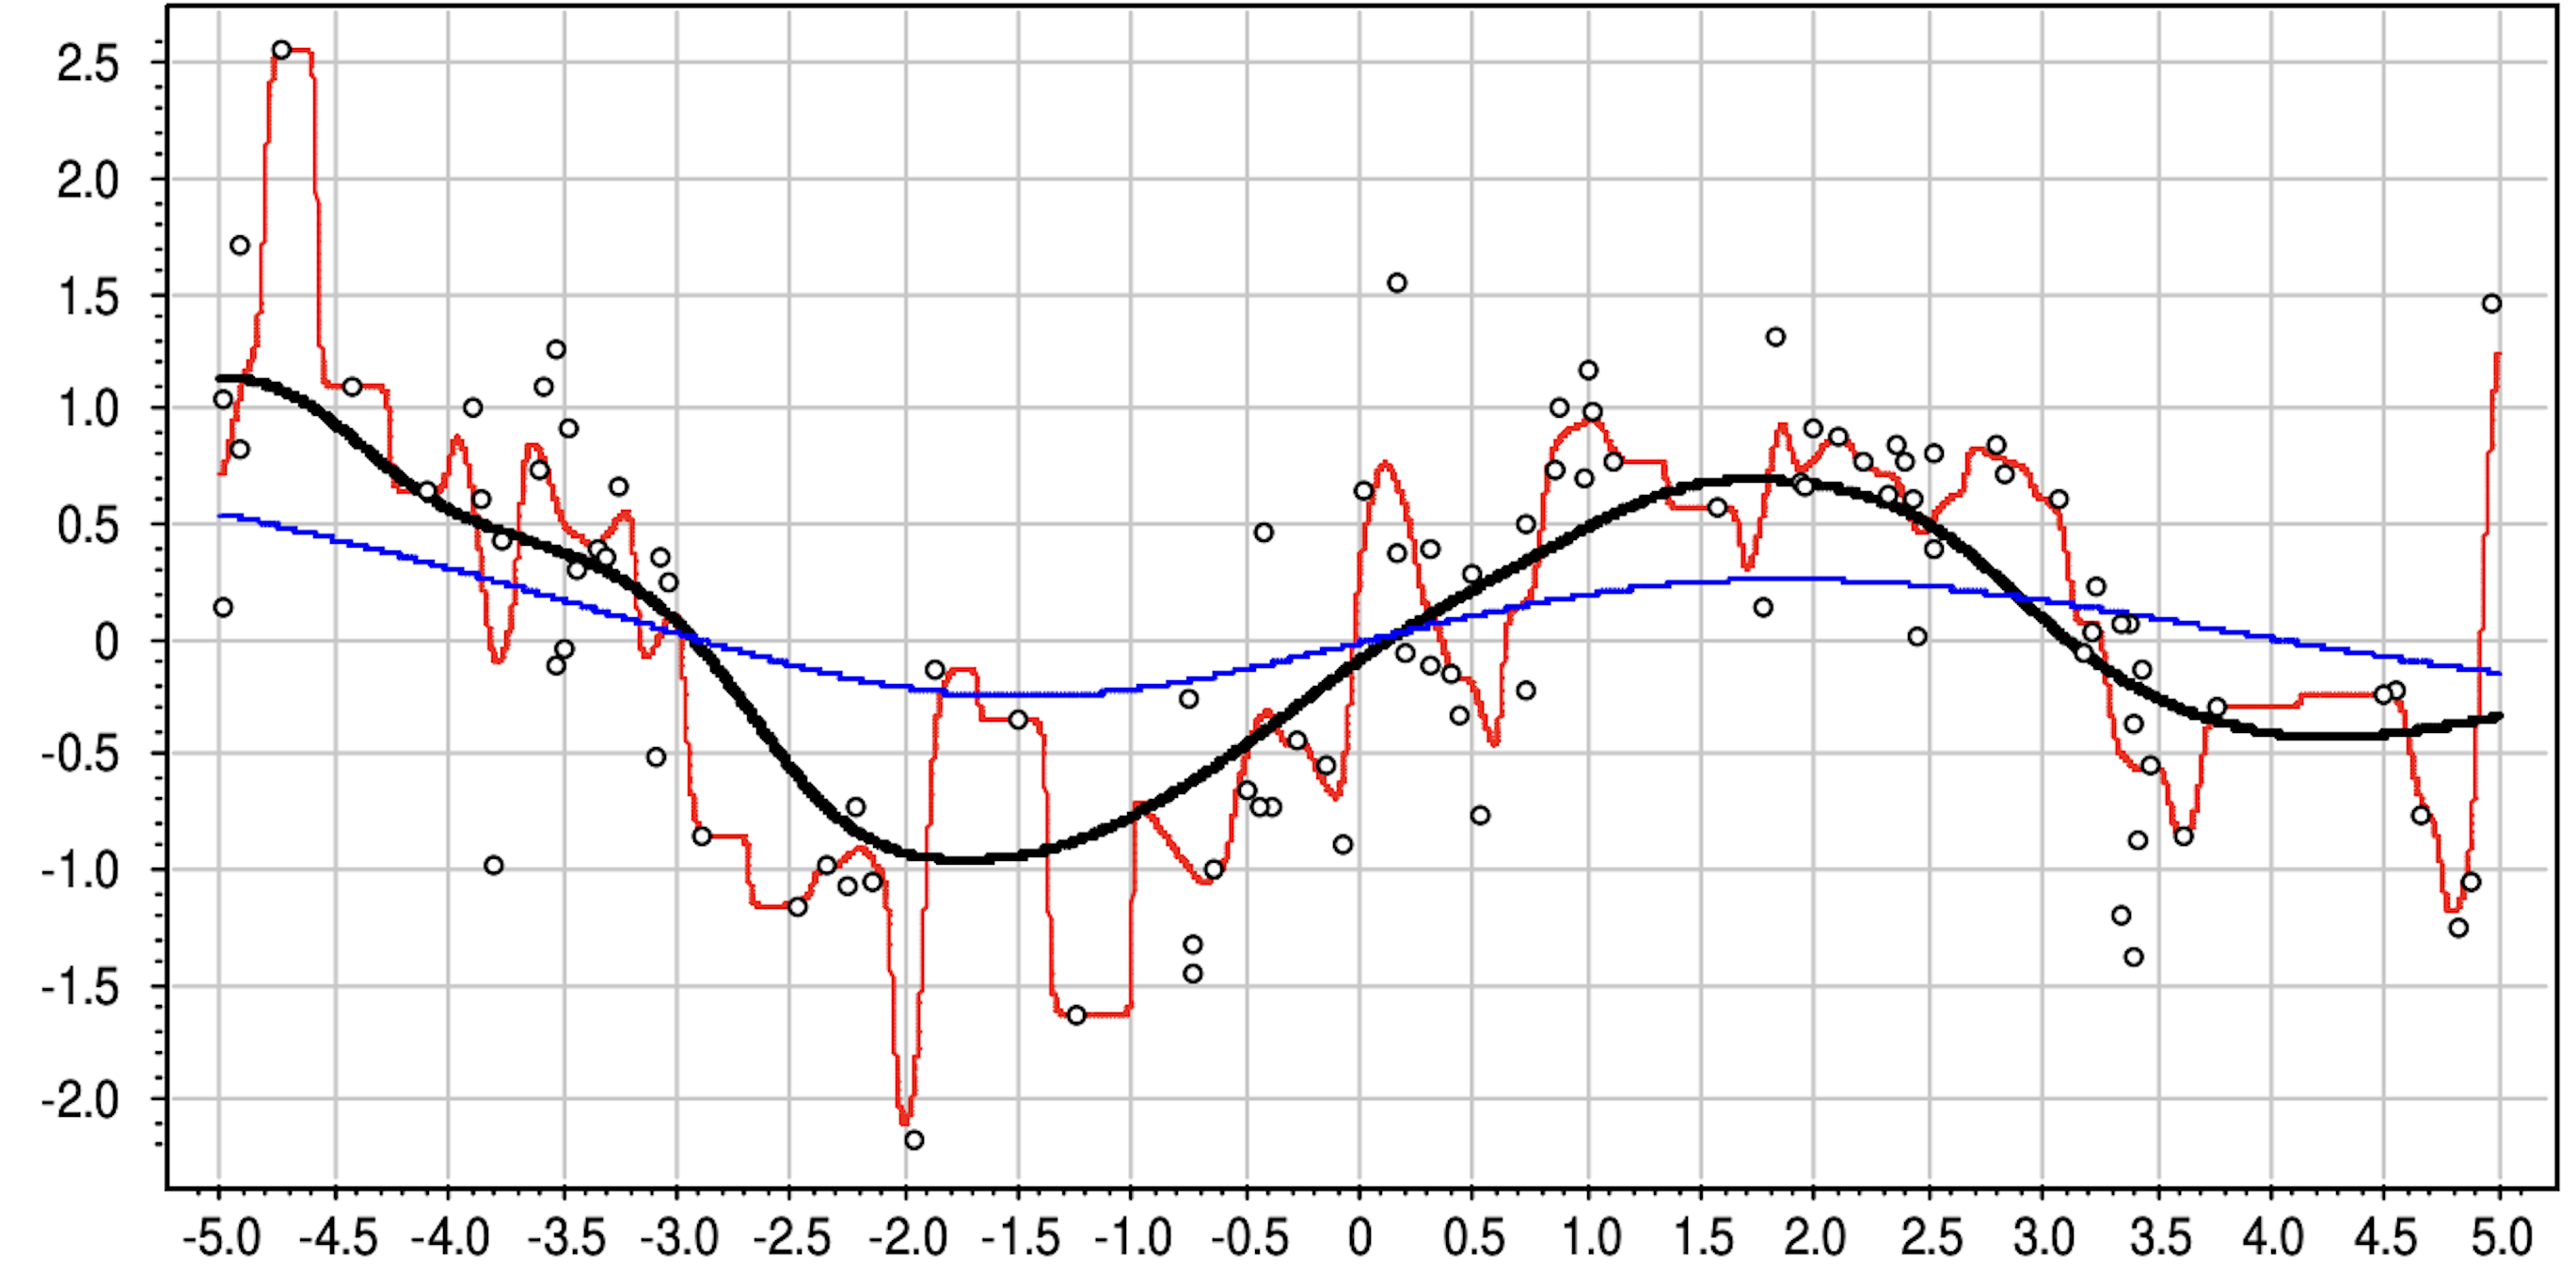
\includegraphics[width=\textwidth]{chapters/metric/images/I2.png}
    \label{fig:kernel_choice}
\end{figure}

\begin{itemize}
    \item Гауссовское ядро \(\Rightarrow\) гладкая аппроксимация
    \item Ширина окна существенно влияет на точность аппроксимации
\end{itemize}

\section*{Выбор ядра \(K\) и ширины окна \(h\)}

\noindent
\(h \in \{\textcolor{red}{0.1}, 1.0, \textcolor{blue}{3.0}\}\), треугольное ядро \(K(r) = (1 - \lvert r \rvert) [{\lvert r \rvert \leq 1}]\). Графики с разными значениями \(h\) при треугольном ядре:
\begin{figure}[ht]
    \centering
    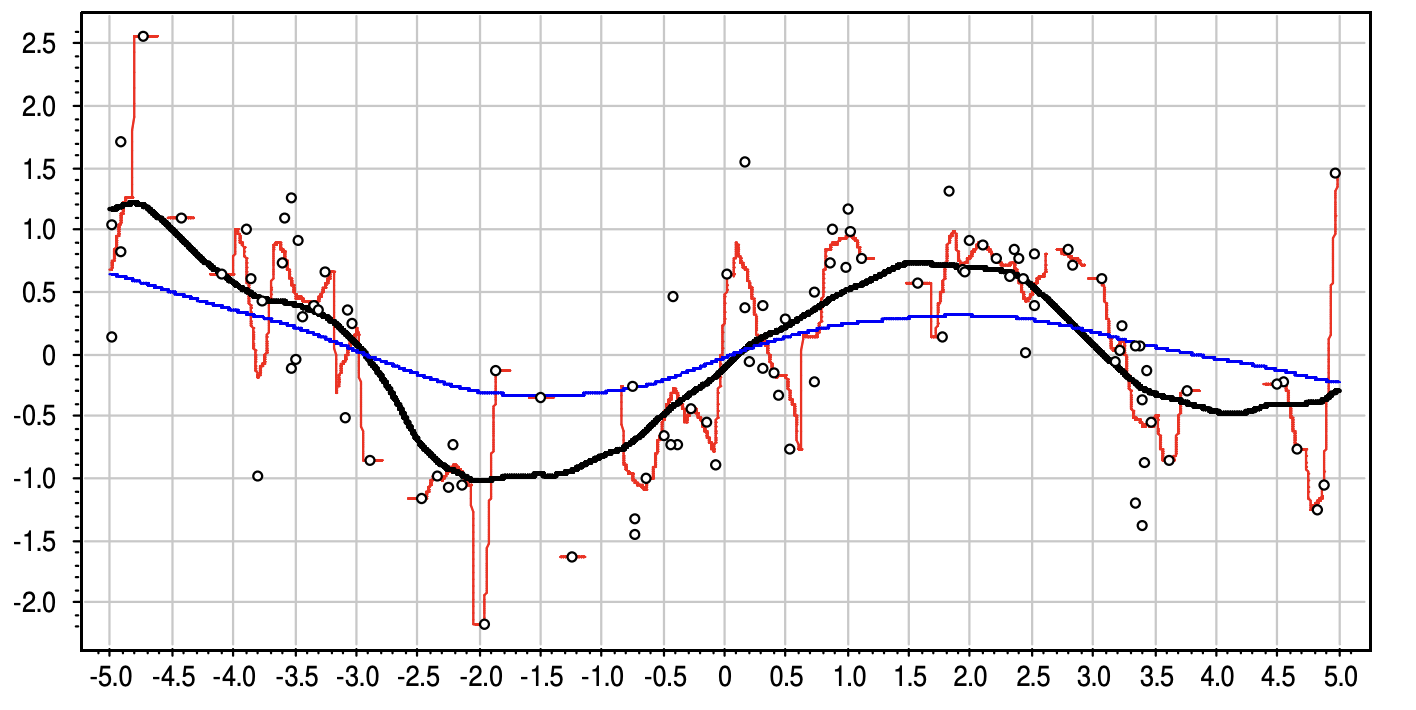
\includegraphics[width=\textwidth]{chapters/metric/images/I3.png}
    \label{fig:kernel_triangle-1}
\end{figure}

\begin{itemize}
    \item Треугольное ядро \(\Rightarrow\) кусочно-линейная аппроксимация
    \item Аппроксимация не определена, если в окне нет точек выборки
\end{itemize}

\section*{Выбор ядра \(K\) и ширины окна \(h\)}

\begin{itemize}
    \item \textbf{Ядро \(K(r)\)}
    \begin{itemize}
        \item существенно влияет на гладкость функции \( a_h(x) \),
        \item слабо влияет на качество аппроксимации.
    \end{itemize}
    \item \textbf{Ширина окна \(h\)}
    \begin{itemize}
        \item существенно влияет на качество аппроксимации.
    \end{itemize}
    \item \textbf{Переменная ширина окна по \(k\) ближайшим соседям:}
    \[
    w_i(x) = K\left( \frac{\rho(x, x_i)}{h(x)} \right), \quad h(x) = \rho(x, x^{(k+1)})
    \]
    где \(x^{(k)}\) — \(k\)-й сосед объекта \(x\).

    \item \textbf{Оптимизация ширины окна по скользящему контролю:}
    \[
    \text{LOO}(h, X^\ell) = \sum_{i=1}^\ell \left( a_h(x_i; X^\ell \setminus \{x_i\}) - y_i \right)^2 \to \min_h
    \]
\end{itemize}

\section*{Проблема выбросов (эксперимент на синтетических данных)}

\noindent
\(\ell = 100\), \(h = 1.0\), гауссовское ядро \(K(r) = \exp(-2r^2)\)

\vspace{0.5em}

{\color{red}Две из 100 точек — выбросы с ординатами \(y_i = 40\) и \(-40\)}

\vspace{0.5em}

{\color{blue}Синяя кривая — выбросов нет}

\begin{align*}
    \centering
    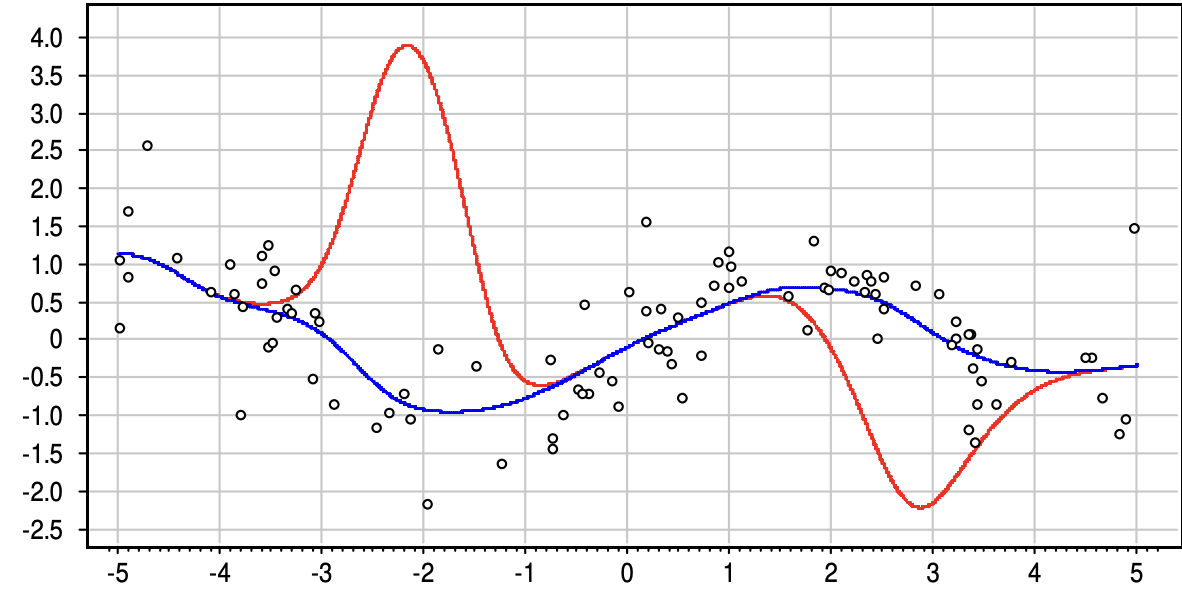
\includegraphics[width=\textwidth]{chapters/metric/images/I4.png}
    \label{fig:kernel_triangle-2}
\end{align*}

\section*{Проблема выбросов и локально взвешенное сглаживание}

\textbf{Проблема выбросов:} точки с большими случайными ошибками \(y_i\) сильно искажают функцию \(a_h(x)\)

\vspace{1em}
\textbf{Основная идея:} \\
чем больше величина ошибки \(\varepsilon_i = \lvert a_h(x_i; X^\ell \setminus \{x_i\}) - y_i \rvert\), \\
тем больше прецедент \((x_i, y_i)\) похож на выброс, \\
тем меньше должен быть его вес \(w_i(x)\).

\vspace{1em}
\textbf{Эвристика:} \\
домножить веса \(w_i(x)\) на коэффициенты \(\gamma_i = \tilde{K}(\varepsilon_i)\), \\
где \(\tilde{K}\) — ещё одно ядро, вообще говоря, отличное от \(K(r)\).

\vspace{1em}
\textbf{Рекомендация:} \\
квартическое ядро \(\tilde{K}(\varepsilon) = K_Q \left( \frac{\varepsilon}{6 \, \mathrm{med}\{\varepsilon_i\}} \right)\), \\
где \(\mathrm{med}\{\varepsilon_i\}\) — медиана вариационного ряда ошибок.

\section*{Алгоритм LOWESS (LOcally WEighted Scatter plot Smoothing)}

\vspace{1em}
\textcolor{blue}{\textbf{Вход:}} \(X^\ell\) — обучающая выборка; \\
\textcolor{blue}{\textbf{Выход:}} коэффициенты \(\gamma_i, \quad i = 1, \ldots, \ell\);

\vspace{1em}
инициализация: \(\gamma_i := 1, \quad i = 1, \ldots, \ell\);

\vspace{1em}
\textcolor{blue}{\textbf{повторять}}
\begin{itemize}
    \item оценки скользящего контроля в каждом объекте:
    \[
    a_i := a_h(x_i; X^\ell \setminus \{x_i\}) = \frac{\sum\limits_{j=1, j \neq i}^{\ell} y_j \gamma_j K\left( \frac{\rho(x_i, x_j)}{h(x_i)} \right)}{\sum\limits_{j=1, j \neq i}^{\ell} \gamma_j K\left( \frac{\rho(x_i, x_j)}{h(x_i)} \right)}, \quad i = 1, \ldots, \ell;
    \]
    \item \(\gamma_i := \tilde{K}(\lvert a_i - y_i \rvert), \quad i = 1, \ldots, \ell;\)
\end{itemize}

\textcolor{blue}{\textbf{пока}} коэффициенты \(\gamma_i\) не стабилизируются;

\section*{Пример работы LOWESS на синтетических данных}

\noindent
\(\ell = 100\), \(h = 1.0\), гауссовское ядро \(K(r) = \exp(-2r^2)\)

\vspace{1em}

Две из 100 точек — выбросы с ординатами \(y_i = 40\) и \(-40\)

\vspace{1em}

В данном случае LOWESS сходится за несколько итераций:
\begin{align*}
    \centering
    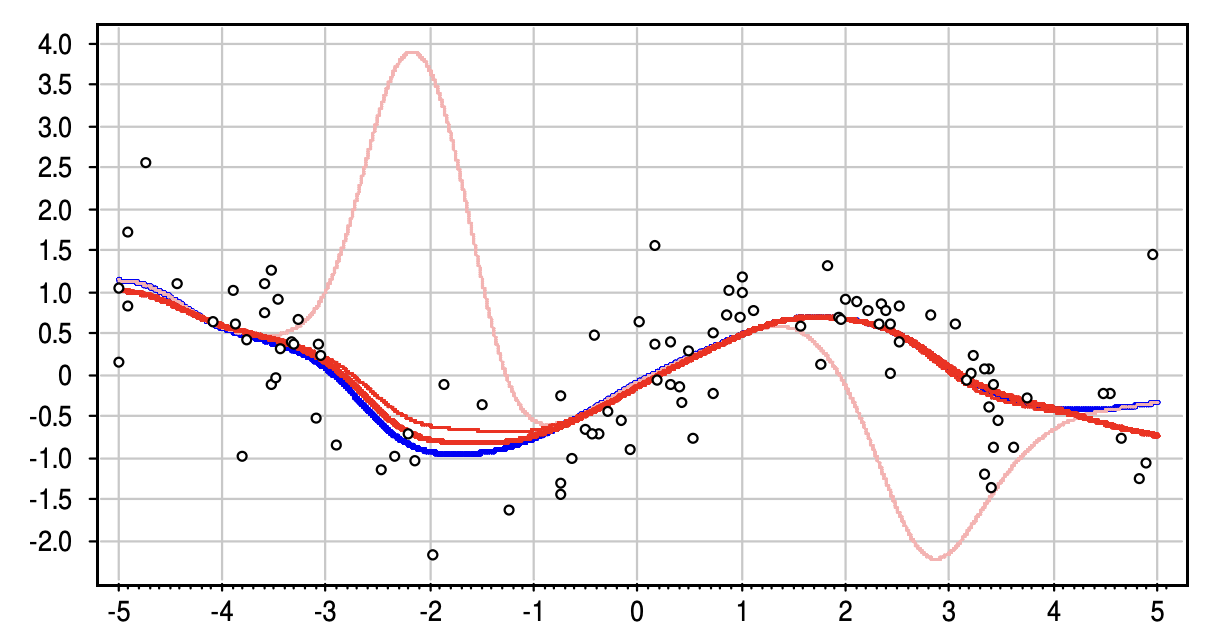
\includegraphics[width=\textwidth]{chapters/metric/images/I5.png}
    \label{fig:kernel_triangle}
\end{align*}

\section{Задачи}
\subsection{Задача 1}
Объясните, как выбор ядра \(K(r)\) влияет на гладкость регрессионной функции \(a_h(x)\). Приведите примеры различных ядер и их влияния.
\subsection{Ответ:}
Ядро \(K(r)\) определяет форму и вес окрестности точки, используемой для оценки регрессионной функции. Гладкие ядра, такие как гауссовское, дают более плавные оценки, в то время как менее гладкие, такие как прямоугольное, приводят к менее сглаженным функциям. Например:

- Гауссовское ядро \(K(r) = \exp(-r^2)\) — даёт плавные, гладкие оценки.

- Треугольное ядро \(K(r) = 1 - \lvert r \rvert\) (при \(\lvert r \rvert \leq 1\)) — более резкое, но все ещё гладкое.

- Прямоугольное ядро \(K(r) = 0.5\) (при \(\lvert r \rvert \leq 1\)) — приводит к кусочно-постоянной функции.

\subsection{Задача 2}
Приведите пример оптимального веса \(w_i(x)\) в алгоритме LOWESS, если известно распределение ошибок в данных. Поясните, как это распределение должно влиять на выбор веса, и почему весовое ядро \(\tilde{K}\) должно учитывать распределение ошибок.

\subsection{Ответ:}
Если ошибка \(\varepsilon_i\) распределена согласно некоторому известному распределению, например нормальному, \( \varepsilon_i \sim \mathcal{N}(0, \sigma^2)\), то весовой коэффициент должен минимизировать дисперсию предсказания. Весовая функция \(\tilde{K}(\varepsilon_i)\) должна убывать, когда \(\varepsilon_i\) отклоняется от некоторого центрального значения (0 для нормального распределения), чтобы уменьшить влияние выбросов:

\[
w_i(x) = \exp\left(-\frac{\varepsilon_i^2}{2\sigma^2}\right)
\]

Этот вес сильнее подавляет ошибки, отклоняющиеся от средней, что уменьшает их влияние на итоговую модель. Выбор весового ядра \(\tilde{K}\) должен учитывать распределение ошибок, чтобы учесть типичные вариации данных.

\subsection{Задача 3}
На основе метода LOWESS предложите способ оценки доверительного интервала для предсказаний. Выведите формулу для доверительного интервала и объясните, как она может быть использована для оценки надежности модели.

\subsection{Ответ:}

\quad 1. Построение модели:

   - Применим LOWESS для построения основной модели, получив предсказанные значения \( \hat{y}_i \) для каждого \(x_i\).

2. Оценка остаточной дисперсии:

   - Вычислим остаточные отклонения \(e_i = y_i - \hat{y}_i\).

   - Оценим дисперсию ошибок \(\sigma^2\) как среднеквадратическое отклонение:

     \[
     \sigma^2 = \frac{1}{n-k} \sum_{i=1}^{n} e_i^2
     \]

   где \(n\) — число точек данных, \(k\) — число параметров (в случае LOWESS, это скорее степень полинома в локальных регрессиях).

3. Построение доверительного интервала:

   - Для каждого предсказанного значения \( \hat{y}_i \) построим доверительный интервал, используя стандартное отклонение остаточных ошибок и критические значения из t-распределения:

     \[
     \hat{y}_i \pm t_{\alpha/2, n-k} \cdot \sqrt{\frac{\sigma^2}{n_i}}
     \]

   где \( t_{\alpha/2, n-k} \) — квантиль t-распределения с уровнем значимости \(\alpha\), и \(n_i\) — эффективное число точек в окрестности \(x_i\) (окрестность, которая использовалась для регрессии, может быть выражена размером окна или числом соседей).

4. Использование доверительных интервалов:

   - Доверительные интервалы позволяют пользователю оценить, насколько "надёжны" предсказанные значения. Узкие интервалы свидетельствуют о высокой уверенности.

   - Визуализация доверительных интервалов на графиках помогает выявлять области, где модель может быть неопределённой или подверженной ошибкам.

\section{Формула Надарая-Ватсона.}
 $X$ -объекты
 $Y$ -ответы
 $X = (x_i, y_i)^l_{i=1}$-обучающая выборка
Будем обозначать $x_i = (x_i^1, ..., x_i^n)$ - вектор признаков объекта $x_i$.

$a(x)= f(x,\theta)$ - параметрическая модель зависимости
$\theta$ -вектор параметров модели

Метод наименьших квадратов (МНК):
\begin{equation*}
    \displaystyle Q(\theta; X^l) =  \sum\limits_{i=1}^l(f(x_i, \theta)-y_i)^2w_i \longrightarrow \min_\theta,
\end{equation*}
где $w(i,x)$ - некоторый вес, отражающий степень важности i-ого объекта. Вес неотрицателен и не возрастает по $i$.


Сложно определить, какую стоит взять параметрическую модель.

\textit{Идея:}
Будем считать, что $f(x_i, \theta)=\theta$,  а $w_i$ зависит от x - т. е. веса объектов задаются в зависимости от того, на каком объекте будет получен объект.
Мы будем обучаться для каждого объекта, на котором хотим получить y.

Тогда:
\begin{equation*}
    \displaystyle Q(\theta; X^l) =  \sum\limits_{i=1}^l(\theta-y_i)^2w(i,x) \longrightarrow \min_\theta,
\end{equation*}
Наконец, положим
\begin{equation*}
    \displaystyle w_i(x) = K\left(\frac{\rho(x, x^{(i)})}{h}\right),
\end{equation*}
где $K(r)$ - невозрастающая функция, определённая на неотрицательных числах, называемая ядром, положительная на отркезке $[0,1]$, $h$ - ширина окна. То есть, чем больше расстояние до $x^{(i)}$, тем меньше оно влияет на x.
\\ Продифференцируем $Q(\theta; X^l)$ по $\theta$ и приравняем получившееся значение 0, и отсюда получим формулу ядерного сглаживания Надарая-Ватсона:
\begin{equation*}
   \textcolor{blue} {\theta(x, X^l)= \frac{\sum\limits_{i=1}^ly_iw_i(x)}{\sum\limits_{i=1}^lw_i(x)}= \frac{\sum\limits_{i=1}^ly_iK\left(\frac{\rho(x, x^{(i)})}{h}\right)}{\sum\limits_{i=1}^lK\left(\frac{\rho(x, x^{(i)})}{h}\right)}}
\end{equation*}

Средневзвешенное значение y на тех объектах, которые близки к x.

Мы видим, что такой метод для каждого объекта $x$ рассматривает только объекты обучающей выборки, находящиеся на расстоянии не больше $h$ от $x$. Причём, чем дальше объект от $x$, тем  меньший вклад он даёт в оценку близости.



\textbf{Обоснование формулы Надарая-Ватсона:}

\textbf{Теорема:}
пусть выполнены следующие условия:
\begin{enumerate}
    \item Выборка $X^l$ простая из совместного распределения $p(x,y)$
    \item ядро $K(r)$ ограничено $\displaystyle\int\limits_{0}^{+\infty} K(r)dr < \infty$,
    $\lim\limits_{r \to \infty}  rK(r) =0$.
    (из этого условия следует, что ядро приводит большие расстояния в 0)
    \item зависимость E(y|x) не имеет вертикальных асимптот

    $E(y^2|x)=\displaystyle\int\limits_{Y} y^2p(y|x)dy < \infty$ при любом $x \in X$
    \item последовательность $h_l$ (ширина окна) убывает с ростом выборки, но не слишком быстро и не слишком медленно
    $\lim\limits_{l\to \infty} h_l=0$,
    $\lim\limits_{l\to \infty} l h_l=0$

    Тогда имеет место сходимость по вероятности:
    $\theta(x, X^l) \xrightarrow{p}E(y|x) $

(здесь Е -мат. ожидание у при условии х)

    в любой точке $x \in X$, в которой E(y|x),  p(x), D(y|x) -непрерывны, p(x)>0
\end{enumerate}

По теореме даже если распределение $p(x,y)$ и E(y|x) не известны, $\theta$ будет стремится к нему с ростом длины обучающей выборки


\textit{Замечание.} Ширина окна отвечает за пере или недообучение,
следовательно сильно влияет на качество аппроксимации.



Для подбора наилучшей модели оптимизируются параматры:
\begin{itemize}
    \item ширина окна $h$;
    \item ядро $K$.
\end{itemize}

 Приведём примеры наиболее часто используемых ядер:
\begin{itemize}
    \item $\displaystyle K_1(r) = (1-r^2)[r\le1]$ - ядро Епанечникова;
    \item $\displaystyle K_2(r) = (1-r^2)^2[r\le1]$ - квартическое ядро;
    \item $\displaystyle K_3(r) = (1-|r|)[r\le1]$ - треугольное ядро;
    \item $\displaystyle K_4(r) = [r\le1]$ - прямоугольное ядро; \item $\displaystyle K_5(r) = e^{-2r^2}$ - гауссовское ядро.
\end{itemize}
\textit{Замечание.} Существует проблема выбросов, при которой точки с большими случайными $y_i$ сильно искажают итоговую функцию. С этим можно справиться, домножив веса $w_i$ на коэффициенты $\gamma_i = K^*(\epsilon_i)$, где $\epsilon_i =|\theta(x_i, X^l)-y_i|$ подразумевается, что из $X^l$ исключили $x_i, K^*$-другое ядро


\textbf{Задача 1.}
Объяснить, почему не стоит брать финитное ядро на неизвестных данных при малой ширине окна h. Объяснить, почему нельзя просто взять большое h, чтобы решить проблему из предыдущего пункта.

\textbf{Ответ:}
При малой ширине окна h и финитном ядре у некоторых точек может не оказаться соседей, попадающих в радиус ядра К. На случай такого события в формулу Надарая-Ватсона в знаменатель добавляют малый член, чтобы не делить на 0.

Если увеличить ширину окна h, то для всех точек с большей вероятностью смогут найтись соседи, но в таком случае точность аппроксимации ухудшится.
\\

\textbf{Задача 2.}  как ядро влияет на гладкость функции? Ответ обосновать.

\textbf{Ответ:}
Будем считать, что ядро не обращается в 0.
Вспомним, что функция, являющаяся результатом деления двух гладких функций, является гладкой.
Сумма гладких функций, умноженных на число- также гладкая функция
Пусть ядро К - гладкое, тогда ${\sum\limits_{i=1}^ly_iK\left(\frac{\rho(x, x^{(i)})}{h}\right)}$ -гладкое, и функция
$\frac{\sum\limits_{i=1}^ly_iK\left(\frac{\rho(x, x^{(i)})}{h}\right)}{\sum\limits_{i=1}^lK\left(\frac{\rho(x, x^{(i)})}{h}\right)}$
будет гладкой

Следовательно, выбор ядра сильно влияет на гладкость.

\textbf{Задача 3.} Имеются следующие данные: x = [1.2, 2.7, 3.1, 4.5, 5.3],  y = [3.5, 1.8, 5.2, 2.1, 4.7].  Необходимо предсказать значение y для x = 2.5, используя формулу Надарая-Ватсона с квартическим ядром и h = 1.


\textbf{Решение:} Для каждой точки из набора данных вычисляем вес $K(\frac{x-x_i}{h})$,

где x = 2.5, h =1,
Суммируем все вычисленные веса и делим каждый вес на эту сумму, чтобы получить нормированные веса.

веса не равны 0 только у точек x=2.7 x=3.1, их веса равны соответственно 0.9216 и 0.4096.

При нормировке получим веса 0.6923 и 0.3077
Предсказание ŷ(2.5) вычисляется как взвешенная сумма значений по уже известной формуле

примерный ŷ(2.5) =2.85


\section{Влияние выбора метрики на качество работы kNN}

Метод \(k\)-ближайших соседей (kNN) является одним из базовых алгоритмов машинного обучения и широко применяется в задачах классификации и регрессии. Этот алгоритм относится к метрическим методам, так как выбор ближайших соседей основывается на измерении расстояний между объектами. Главным фактором, определяющим качество модели, является выбор метрики расстояния, так как она определяет, какие объекты считаются «похожими».

\subsection{Сущность метода k-ближайших соседей}

Алгоритм \(k\)-ближайших соседей работает следующим образом:
\begin{enumerate}
    \item Для нового объекта вычисляется расстояние до всех объектов обучающей выборки.
    \item Выбираются \(k\) ближайших объектов в соответствии с выбранной метрикой.
    \item Класс нового объекта определяется на основе классов выбранных соседей (например, по принципу большинства для задач классификации).
    \item В задачах регрессии целевое значение нового объекта вычисляется как среднее (или взвешенное среднее) значений соседей.
\end{enumerate}

Ключевым аспектом метода является расстояние, вычисляемое на основе метрики, которая влияет на работу алгоритма, в том числе на точность и устойчивость модели.

\subsection{Популярные метрики расстояния}

\begin{enumerate}
    \item \textbf{Евклидова метрика} (\(L2\)-норма):
    Одна из самых популярных метрик, измеряющая геометрическое расстояние между точками в пространстве.
    Формула:
    \[
    d(x, y) = \sqrt{\sum_{i=1}^{n}(x_i - y_i)^2}
    \]
    Особенности:
    \begin{itemize}
        \item Подходит для данных, где все признаки одинаково масштабированы.
        \item Чувствительна к выбросам, так как квадрат отклонения значительно увеличивает вклад большого расхождения.
    \end{itemize}

    \item \textbf{Манхэттенская метрика} (\(L1\)-норма):
    Измеряет расстояние как сумму абсолютных разностей координат.
    Формула:
    \[
    d(x, y) = \sum_{i=1}^{n}|x_i - y_i|
    \]
    Особенности:
    \begin{itemize}
        \item Лучше подходит для разреженных данных.
        \item Менее чувствительна к выбросам по сравнению с Евклидовой метрикой.
    \end{itemize}

    \item \textbf{Метрика Минковского}:
    Обобщение Евклидовой и Манхэттенской метрик.
    Формула:
    \[
    d(x, y) = \left(\sum_{i=1}^{n}|x_i - y_i|^p\right)^{\frac{1}{p}}
    \]
    Особенности:
    \begin{itemize}
        \item При \(p=2\) совпадает с Евклидовой метрикой, при \(p=1\) — с Манхэттенской.
        \item Позволяет гибко настраивать степень влияния больших отклонений через параметр \(p\).
    \end{itemize}

    \item \textbf{Косинусное расстояние}:
    Измеряет угол между векторами, игнорируя их длину.
    Формула:
    \[
    d(x, y) = 1 - \frac{\langle x, y \rangle}{\|x\| \cdot \|y\|}
    \]
    Особенности:
    \begin{itemize}
        \item Часто применяется для текстовых данных (например, векторов TF-IDF).
        \item Устойчиво к изменениям масштаба векторов.
    \end{itemize}

    \item \textbf{Метрика Чебышёва}:
    Учитывает максимальное различие по одной из координат.
    Формула:
    \[
    d(x, y) = \max_{i}|x_i - y_i|
    \]
    Особенности:
    \begin{itemize}
        \item Удобна для задач, где критически важно учитывать наибольшее расхождение.
        \item Формирует кубические границы ближайших соседей.
    \end{itemize}
\end{enumerate}

\subsection{Влияние выбора метрики на качество работы модели}

Выбор метрики может значительно изменить поведение алгоритма \(k\)-ближайших соседей. Основные факторы влияния:

\begin{enumerate}
    \item \textbf{Геометрия данных:}
    Разные метрики формируют разные границы классов. Например, Евклидова метрика создает округлые границы, а Манхэттенская — прямоугольные. В задачах с нелинейными разделяющими гиперплоскостями может потребоваться комбинированный подход или нестандартные метрики.

    \item \textbf{Масштаб признаков:}
    Метрики, такие как Евклидова, чувствительны к различиям в масштабе признаков. Например, если один признак имеет диапазон [0, 1], а другой — [0, 1000], последний будет доминировать. Для решения этой проблемы применяется нормализация или стандартизация данных.

    \item \textbf{Шум и выбросы:}
    Метрики по-разному реагируют на шум. Евклидова метрика чувствительна к выбросам, так как квадратичное расстояние значительно увеличивается для больших расхождений. Метрики, такие как Манхэттенская или косинусное расстояние, менее чувствительны к шуму.

    \item \textbf{Высокая размерность:}
    В задачах с большим количеством признаков (проблема «проклятия размерности») расстояния между всеми объектами становятся примерно одинаковыми. Это снижает различимость ближайших соседей, что делает выбор метрики критически важным.

    \item \textbf{Специфика задачи:}
    Например, для задач обработки текстов косинусная метрика часто оказывается лучше, так как она учитывает только направление векторов, игнорируя их длину. Для задач с пространственными данными чаще применяются Евклидова или Манхэттенская метрика.
\end{enumerate}

\subsection{Примеры задач}

\begin{enumerate}
    \item \textbf{Теоретическая задача:}
    Рассмотрите два набора данных из двух классов, представленных точками на плоскости.
    Постройте границы разделения классов при использовании:
    \begin{itemize}
        \item Евклидовой метрики,
        \item Манхэттенской метрики.
    \end{itemize}
    Объясните, как выбор метрики влияет на форму границ.

    \item \textbf{Практическая задача:}
    Используя набор данных \texttt{Iris}, обучите модель \(k\)-ближайших соседей с Евклидовой, Манхэттенской и косинусной метриками. Сравните метрики качества (точность, F1-меру) и сделайте вывод о том, какая метрика работает лучше и почему.

    \item \textbf{Исследовательская задача:}
    Для синтетических данных с перекрывающимися классами разработайте алгоритм выбора оптимальной метрики с использованием кросс-валидации. Постройте графики зависимости точности от параметра \(k\) для разных метрик.
\end{enumerate}

\subsection{Заключение}

Выбор метрики расстояния является ключевым фактором, определяющим качество работы метода \(k\)-ближайших соседей. Оптимальная метрика зависит от природы данных, задачи и требований к точности и устойчивости модели. Для улучшения результатов рекомендуется проводить предварительный анализ данных, нормализацию признаков и тестирование нескольких метрик с использованием кросс-валидации.

\section{Более быстрые оптимизации kNN.}

Описанный в пункте 4.3 тип KNN называется Brute-Force, поскольку в нём используется метод полного перебора для поиска ближайших соседей, что делает его простым в реализации, но слишком медленным при работе с большим объемом данных. Для решения данной проблемы в реализации scikit-learn предусмотрены более продвинутые методы, основанные на бинарных деревьях, что позволяет получить значительный прирост в производительности.

\subsection{BallTree}
BallTree — это древовидная структура, в основе которой лежит разбиение исходного пространства данных на вложенные гиперсферы, что позволяет более эффективно отсекать большие области пространства, в которых отсутствуют ближайшие соседи для точек. В большинстве случаев такой алгоритм подходит для данных с произвольной метрикой расстояния.  
  
Построение BallTree состоит из следующих шагов:  

\begin{enumerate}
    \item   
из множества точек выбирается одна случайным образом и для неё находится самая дальняя точка;
\item
далее все точки разбиваются на гиперсферы (узлы) по ближайшему расположению к двум точкам из шага 1;
\item
затем данный процесс повторяется рекурсивно для каждой гиперсферы, пока в ней не останется определённое количество точек или не будет достигнута заданная глубина дерева.
\end{enumerate}
При поиске k-ближайших соседей для новой точки, алгоритм сравнивает расстояние от заданной точки до центра каждого дочернего узла и оставляет лишь те, в которых данное расстояние меньше радиуса узлов.

Для оценки качества полученной древовидной структуры и её дальнейшей оптимизации очень полезной будет информация о пересекающихся гиперсферах (узлах) A и B в метрике M, расстояние между которыми можно определить следующим образом:

\[
d_M(A, B) = \max(0, d_M(c_A, c_{B}) - r_A - r_{B})
\]

где $c_A$ и $c_{B}$ — центры сфер, а $r_A$ и $r_B$ — их радиусы.


В данном случае оптимизация BallTree с учётом пересекающихся гиперсфер (узлов) может включать в себя следующие подходы:

балансировка дерева: поскольку пересечение гиперсфер может указывать на несбалансированность дерева, перебалансировка его узлов позволяет улучшить эффективность поиска, минимизируя количество посещаемых узлов;

выбор оптимального размера листа: в случае сильного пересечения гиперсфер, увеличение размера листа может уменьшить количество узлов, что также ускорит поиск;

слияние узлов: полезно при значительном пересечении, что также уменьшает их общее количество и используется в предыдущих пунктах;

выбор порядка обхода: информация о структуре пересечения может сделать более эффективным порядок посещаемых узлов, начиная проверку с наиболее вероятных кандидатов.

Стоит отметить, что описанные методы оптимизации плюс-минус похожим образом могут быть применимы и для алгоритма ниже.

\subsection{KD-Tree}
KD-Tree (k-dimensional tree) — ещё одна древовидная структура, отдалённо напоминающая BallTree, однако в данном случае используются гиперплоскости для разбиения точек вместо гиперсфер, что позволяет также эффективно оставлять лишь те области пространства данных, в которых могут присутствовать ближайшие соседи. Обычно KD-Tree больше подходит для данных с евклидовой или манхэттенской метрикой расстояния.

Построение KD-Tree состоит из следующих шагов:

1) из множества точек выбирается одна из координат (обычно поочередно для каждого уровня дерева, но можно и случайным образом) и по ней вычисляется медиана;

2) далее все точки разбиваются на два узла (подмножества) по отношению к медиане: на те, у которых значение выбранной координаты меньше либо равно медиане, и на те, у которых больше;

3) данный процесс повторяется рекурсивно для каждого узла, пока в нём не останется определённое количество точек или не будет достигнута заданная глубина дерева.

При поиске ближайших соседей для новой точки, алгоритм сравнивает значение заданной точки с медианой в каждом узле, выбирая таким образом ближайшее подпространство, которое будет листом с ближайшими соседями. Возвращаясь обратно к корню, алгоритм будет сравнивать точки в текущем узле с ближайшими соседями и обновлять их значения в случае нахождения более близких к заданной точке.

\subsection{Примеры задач}

% \begin{enumerate}
%     \item
\textbf{Задача 1.}
У вас есть два набора данных:

  Набор данных A: 10 миллионов точек в 5-мерном пространстве с использованием Евклидовой метрики.
  
  Набор данных B: 1 миллион точек в 10-мерном пространстве с кастомной метрикой расстояния.
Вопросы:

Какую структуру данных (KD-Tree или BallTree) вы выберете для каждого набора данных? Объясните ваш выбор.
Как влияет размерность пространства на эффективность KD-Tree?\\
\textbf{Ответ:}

Для набора данных A оптимально использовать KD-Tree, так как он хорошо работает с Евклидовой метрикой, особенно в пространствах с небольшой размерностью.
Для набора данных B лучше подходит BallTree, так как он поддерживает произвольные метрики и может быть эффективнее в высоких размерностях.  

С увеличением размерности эффективность KD-Tree значительно снижается из-за проклятия размерности: гиперплоскости разбиения теряют свою полезность, и увеличивается количество узлов, которые нужно проверять.\\
\\
% \end{enumerate}
\textbf{Задача 2.}
Имеется 2D-набор данных с точками:\\ 
(2,3), (5,4), (9,6), (4,7), (8,1), (7,2)
\begin{enumerate}
    \item Постройте KD-Tree для этих точек.
    \item Какие оптимизации можно применить к этому дереву, если оно оказалось несбалансированным?
\end{enumerate}
\textbf{Ответ:}
\begin{enumerate}
    \item Построение дерева:
    \begin{itemize}
        \item Выбор корня: координата \(x\), медиана по \(x\) \( \rightarrow \) точка \((7, 2)\).
        \item Левое поддерево (\(x < 7\)): медиана по \(y\) \( \rightarrow \) точка \((5, 4)\).
        \begin{itemize}
            \item Левый потомок: \((2, 3)\).
            \item Правый потомок: \((4, 7)\).
        \end{itemize}
        \item Правое поддерево (\(x > 7\)): медиана по \(y\) \( \rightarrow \) точка \((9, 6)\).
        \begin{itemize}
            \item Левый потомок: \((8, 1)\).
        \end{itemize}
    \end{itemize}
    Итоговое дерево:

            \[
\begin{array}{c}
    (7, 2)\\
    \downarrow\\
    \begin{array}{cc}
        \text{} & \text{} \\
        \begin{array}{c}
            (5, 4) \\
            \downarrow \\
            \begin{array}{cc}
                (2, 3) & (4, 7)
            \end{array}
        \end{array}
        &
        \begin{array}{c}
            (9, 6) \\
            \downarrow \\
            (8, 1)
        \end{array}
    \end{array}
\end{array}
\]
    \item Оптимизации:
    \begin{itemize}
        \item Если дерево несбалансировано, можно:
        \begin{itemize}
            \item Перестроить дерево, используя медиану всех точек на каждом уровне.
            \item Увеличить размер листов (количество точек в узле) для уменьшения глубины дерева.
        \end{itemize}
    \end{itemize}
\end{enumerate}

\section*{Задача 3: Поиск ближайшего соседа с использованием BallTree}

Дано: гиперсферы в 3D-пространстве, центры \((1, 1, 1)\), \((4, 4, 4)\), радиусы \(r_1 = 2\), \(r_2 = 3\). Найдите ближайшего соседа для точки \((2, 2, 2)\), используя алгоритм BallTree.\\
\textbf{Решение:}
\begin{enumerate}
    \item Вычисляем расстояние от точки до центров гиперсфер:
    \[
    d((2, 2, 2), (1, 1, 1)) = \sqrt{(2-1)^2 + (2-1)^2 + (2-1)^2} = \sqrt{3} \approx 1.73
    \]
    \[
    d((2, 2, 2), (4, 4, 4)) = \sqrt{(2-4)^2 + (2-4)^2 + (2-4)^2} = \sqrt{12} \approx 3.46
    \]
    \item Сравниваем с радиусами:
    \begin{itemize}
        \item Точка \((2, 2, 2)\) находится внутри гиперсферы с центром \((1, 1, 1)\), так как \(1.73 < 2\).
        \item Точка не входит в гиперсферу с центром \((4, 4, 4)\), так как \(3.46 > 3\).
    \end{itemize}
\end{enumerate}

\textbf{Ответ:} Ближайший сосед — точка в гиперсфере с центром \((1, 1, 1)\).

\section{Расстояние Махаланобиса в метрических методах классификации и регрессии}

Метрики являются фундаментальными инструментами в задачах классификации и регрессии, основанных на сходстве или расстоянии между объектами. Они определяют, как мы измеряем "близость" между парами объектов в пространстве признаков.

Расстояние Махаланобиса является обобщением Евклидова расстояния, которое учитывает не только разности значений признаков, но и статистические свойства данных, такие как дисперсии и корреляции между признаками. Это делает его особенно полезным в случае многомерных данных с неоднородной структурой.

\subsection{Определение:}

Расстояние Махаланобиса между вектором признаков объекта \( \mathbf{x} \) и средним вектором \( \mathbf{\mu} \) определяется как:

\[
d(\mathbf{x}, \mathbf{\mu}) = \sqrt{ (\mathbf{x} - \mathbf{\mu})^\top \mathbf{S}^{-1} (\mathbf{x} - \mathbf{\mu}) }
\]
\newline
где:
\newline
- \( \mathbf{x} \) — вектор признаков объекта, \newline
- \( \mathbf{\mu} \) — вектор средних значений признаков (например, центра кластера или класса), \newline
- \( \mathbf{S} \) — ковариационная матрица признаков, \newline
- \( \mathbf{S}^{-1} \) — обратная матрица к \( \mathbf{S} \), \newline
- \( (\mathbf{x} - \mathbf{\mu})^\top \) — транспонированный вектор разностей. \newline

\subsection{Преимущества расстояния Махаланобиса:}

\begin{enumerate}
    \item Расстояние Махаланобиса не зависит от масштаба признаков, что устраняет необходимость в предварительной нормализации или стандартизации данных.

    \item Метрика учитывает корреляции между признаками, что позволяет более точно измерять расстояние в пространстве, где признаки взаимосвязаны.

    \item Она адаптируется к распределению данных, отражая их внутреннюю структуру и дисперсию, что может улучшить результаты в задачах классификации и кластеризации.
\end{enumerate}

\subsection{Недостатки расстояния Махаланобиса:}

\begin{enumerate}
    \item Необходимо вычислять ковариационную матрицу \( \mathbf{S} \)  и обратную матрицу \( \mathbf{S}^{-1} \), что является дорогостоящей операцией, особенно при высокой размерности данных.

    \item Для точной оценки ковариационной матрицы требуется достаточно большой объём данных, число наблюдений должно значительно превышать число признаков.

    \item Если ковариационная матрица не обратима (например, из-за линейной зависимости между признаками или недостаточного числа наблюдений), то невозможно напрямую вычислить \( \mathbf{S}^{-1} \).

    \item Выбросы могут сильно искажать оценку ковариационной матрицы и средних значений, что приводит к неправильному вычислению расстояний.

    \item Сложности в интерпретации: Поскольку расстояние учитывает сложные связи в данных, интерпретация значений может быть менее интуитивной по сравнению с Евклидовым расстоянием.
\end{enumerate}

\subsection{Практические аспекты использования:}

\begin{enumerate}
    \item Регуляризация ковариационной матрицы: Для решения проблем с вырожденностью часто применяется добавление небольшого значения к диагональным элементам ковариационной матрицы (тирихоновская регуляризация).

    \item Понижение размерности: Можно использовать методы понижения размерности (например, анализ главных компонентов) для уменьшения вычислительной нагрузки и устранения мультиколлинеарности.

    \item Отбор признаков: Исключение избыточных или некоррелированных признаков может улучшить оценку ковариационной матрицы и качество метрики.
\end{enumerate}

\subsection{Применение в методах классификации и регрессии}

\begin{enumerate}
    \item Классификация по ближайшим соседям (k-NN): Использование расстояния Махаланобиса вместо Евклидова может улучшить качество классификации в случаях, когда признаки имеют различные масштабы или коррелированы.

    \item Дискриминантный анализ: В линейном дискриминантном анализе (LDA) расстояние между классами измеряется с помощью расстояния Махаланобиса, что позволяет учитывать разброс и ориентацию классов в пространстве признаков.

    \item Обнаружение выбросов: Объекты с большим расстоянием Махаланобиса от центра распределения могут рассматриваться как выбросы.
\end{enumerate}

\subsection{Задачи}

\textbf{Задача 1: Использование расстояния Махаланобиса в классификации k-NN}

Вы применяете метод классификации k-ближайших соседей (k-NN) для разделения объектов на два класса: Класс A и Класс B. У каждого класса известны средние векторы признаков и ковариационные матрицы:

Класс A:
\[
\mathbf{\mu}_A = \begin{bmatrix} 2 \\ 2 \end{bmatrix}, \quad \mathbf{S}_A = \begin{bmatrix} 2 & 0 \\ 0 & 2 \end{bmatrix}
\]

Класс B:
\[
\mathbf{\mu}_B = \begin{bmatrix} 5 \\ 5 \end{bmatrix}, \quad \mathbf{S}_B = \begin{bmatrix} 1 & 0 \\ 0 & 1 \end{bmatrix}
\]

Новый объект имеет признаки \( \mathbf{x} = \begin{bmatrix} 4 \\ 4 \end{bmatrix} \).

Вычислите расстояния Махаланобиса от объекта \( \mathbf{x} \) до каждого класса и определите, к какому классу следует отнести данный объект.

\textbf{Решение:}

1. Расстояние до Класса A:

- Вычисляем разность:
  \[
  \mathbf{x} - \mathbf{\mu}_A = \begin{bmatrix} 4 - 2 \\ 4 - 2 \end{bmatrix} = \begin{bmatrix} 2 \\ 2 \end{bmatrix}
  \]
- Находим обратную ковариационную матрицу \( \mathbf{S}_A^{-1} \):
  \[
  \mathbf{S}_A^{-1} = \begin{bmatrix} \frac{1}{2} & 0 \\ 0 & \frac{1}{2} \end{bmatrix}
  \]
- Вычисляем расстояние:
  \[
  d_A = \sqrt{ (\mathbf{x} - \mathbf{\mu}_A)^\top \mathbf{S}_A^{-1} (\mathbf{x} - \mathbf{\mu}_A) } = \sqrt{ \begin{bmatrix} 2 & 2 \end{bmatrix} \begin{bmatrix} \frac{1}{2} & 0 \\ 0 & \frac{1}{2} \end{bmatrix} \begin{bmatrix} 2 \\ 2 \end{bmatrix} } = \sqrt{ (2)(1) + (2)(1) } = \sqrt{4} = 2
  \]

2. Расстояние до Класса B:

- Вычисляем разность:
  \[
  \mathbf{x} - \mathbf{\mu}_B = \begin{bmatrix} 4 - 5 \\ 4 - 5 \end{bmatrix} = \begin{bmatrix} -1 \\ -1 \end{bmatrix}
  \]
- Обратная ковариационная матрица \( \mathbf{S}_B^{-1} \) уже известна, так как \( \mathbf{S}_B \) — единичная матрица:
  \[
  \mathbf{S}_B^{-1} = \begin{bmatrix} 1 & 0 \\ 0 & 1 \end{bmatrix}
  \]
- Вычисляем расстояние:
  \[
  d_B = \sqrt{ (\mathbf{x} - \mathbf{\mu}_B)^\top \mathbf{S}_B^{-1} (\mathbf{x} - \mathbf{\mu}_B) } = \sqrt{ (-1)^2 + (-1)^2 } = \sqrt{1 + 1} = \sqrt{2} \approx 1{,}414
  \]

3. В итоге:

Поскольку \( d_B < d_A \), объект \( \mathbf{x} \) принадлежит Классу B.



\textbf{Задача 2: Обнаружение аномалий с помощью расстояния Махаланобиса}

В задаче обнаружения мошеннических транзакций используются два признака: сумма покупки (\( X_1 \)) и количество товаров (\( X_2 \)). Для нормальных транзакций известно:

- Средний вектор:
  \[
  \mathbf{\mu} = \begin{bmatrix} 100 \\ 10 \end{bmatrix}
  \]
- Ковариационная матрица:
  \[
  \mathbf{S} = \begin{bmatrix} 400 & 0 \\ 0 & 4 \end{bmatrix}
  \]

Новая транзакция имеет значения \( \mathbf{x} = \begin{bmatrix} 160 \\ 14 \end{bmatrix} \).

Вычислите расстояние Махаланобиса и определите, является ли эта транзакция аномальной, используя пороговое значение \( d_{\text{порог}} = 3 \).

\textbf{Решение:}

1. Вычисляем разность:
\[
\mathbf{x} - \mathbf{\mu} = \begin{bmatrix} 160 - 100 \\ 14 - 10 \end{bmatrix} = \begin{bmatrix} 60 \\ 4 \end{bmatrix}
\]

2. Находим обратную ковариационную матрицу \( \mathbf{S}^{-1} \):
\[
\mathbf{S}^{-1} = \begin{bmatrix} \frac{1}{400} & 0 \\ 0 & \frac{1}{4} \end{bmatrix}
\]

3. Вычисляем расстояние:
\[
d = \sqrt{ (\mathbf{x} - \mathbf{\mu})^\top \mathbf{S}^{-1} (\mathbf{x} - \mathbf{\mu}) } = \sqrt{ (60)^2 \times \frac{1}{400} + (4)^2 \times \frac{1}{4} } = \sqrt{ \frac{3600}{400} + \frac{16}{4} } = \sqrt{9 + 4} = \sqrt{13} \approx 3{,}606
\]

4. Поскольку \( d = 3{,}606 > d_{\text{порог}} = 3 \), транзакция считается аномальной.

\textbf{Задача 3: Выбор метрики расстояния при наличии коррелированных признаков}

Вы работаете с набором данных, содержащим два признака: \( X_1 \) и \( X_2 \). При анализе данных вы обнаружили, что признаки \( X_1 \) и \( X_2 \) имеют сильную положительную корреляцию.

Вы планируете использовать метод k-ближайших соседей (k-NN) для классификации новых объектов. Возникает вопрос: какую метрику расстояния следует использовать — Евклидово расстояние или расстояние Махаланобиса? Объясните свой выбор.

\textbf{Решение:}

Предполагаемые рассуждения:

  - Поскольку признаки \( X_1 \) и \( X_2 \) сильно коррелированы, это означает, что они содержат избыточную информацию. Изменения в одном признаке сопровождаются изменениями в другом.

- При использовании Евклидова расстояния каждый признак рассматривается независимо, без учета корреляции. Это может привести к тому, что влияние коррелированных признаков будет преувеличено, и объекты будут казаться более далекими друг от друга вдоль направления корреляции.

- Расстояние Махаланобиса учитывает ковариацию между признаками. За счет включения ковариационной матрицы оно корректирует влияние коррелированных признаков, "сжимая" пространство вдоль направления корреляции.

Вывод:

В данном случае целесообразнее использовать расстояние Махаланобиса, так как оно учитывает корреляцию между признаками и обеспечивает более точное измерение сходства между объектами. Это улучшит качество классификации методом k-NN, так как позволит корректно определять ближайших соседей основываясь на истинной структуре данных.


\newpage

\section{Профиль компактности и оценка обобщающей способности}

Пусть стоит задача улучшения алгоритма 1NN. Этого можно добиться, оставив из выборки только нужные  элементы, то есть произвести выбор эталонных элементов. Для такого выбора необходимо выполнить минимизацию CCV.


\subsection{CCV}

\noindent
\textbf{Полный скользящий контроль}  (complete cross-validation, CCV):

\begin{equation*}
	\operatorname{CCV}\left(X^L\right)=\frac{1}{C_L^{\ell}} \sum_{X^{\ell} \sqcup X^k} \frac{1}{k} \sum_{x_i \in X^k}\left[a\left(x_i ; X^{\ell}\right) \neq y_i\right]
\end{equation*}

\noindent
- частота ошибок алгоритма на контрольной выборке $X^k$, усреднённая по всем $C_L^{\ell}$ разбиениям выборки $X^L=X^{\ell} \sqcup X^k$ на обучающую подвыборку $X^{\ell}$ и контрольную $X^k$. \\

\noindent
Для дальнейших рассуждений введем понятие профиля компактности.


\subsection{Профиль компактности}

\noindent
\textbf{Профиль компактности} выборки $X^L$ - это функция доли объектов $x_i$, у которых $m$-й сосед $x_i^{(m)}$ лежит в другом классе: $$ \begin{gathered} \Pi(m)=\frac{1}{L} \sum_{i=1}^L\left[y_i \neq y_i^{(m)}\right] ; \quad m=1, \ldots, L-1, \\ x_i^{(m)}-m \text {-й сосед объекта } x_i \text { среди } X^L ; \\ y_i^{(m)}-\text { ответ на } m \text {-м соседе объекта } x_i . \end{gathered} $$


\subsection{CCV для метода 1NN}

\noindent
С учетом введенного $\Pi(m)$ справедлива следующая теорема о точном выражении CСV для метода 1NN:

\begin{equation*}
	\operatorname{CCV}\left(X^L\right)=\sum_{m=1}^k \Pi(m) \frac{C_{L-1-m}^{\ell-1}}{C_{L-1}^{\ell}} .
\end{equation*}

\noindent
Нетрудно заметить, что CСV при длине выборки равной 1 совпадает с LOO (leave-one-out).


\subsection{Пример профилей компактности}

\noindent
Проанализируем графики.

\begin{figure}[ht]
	\centering
	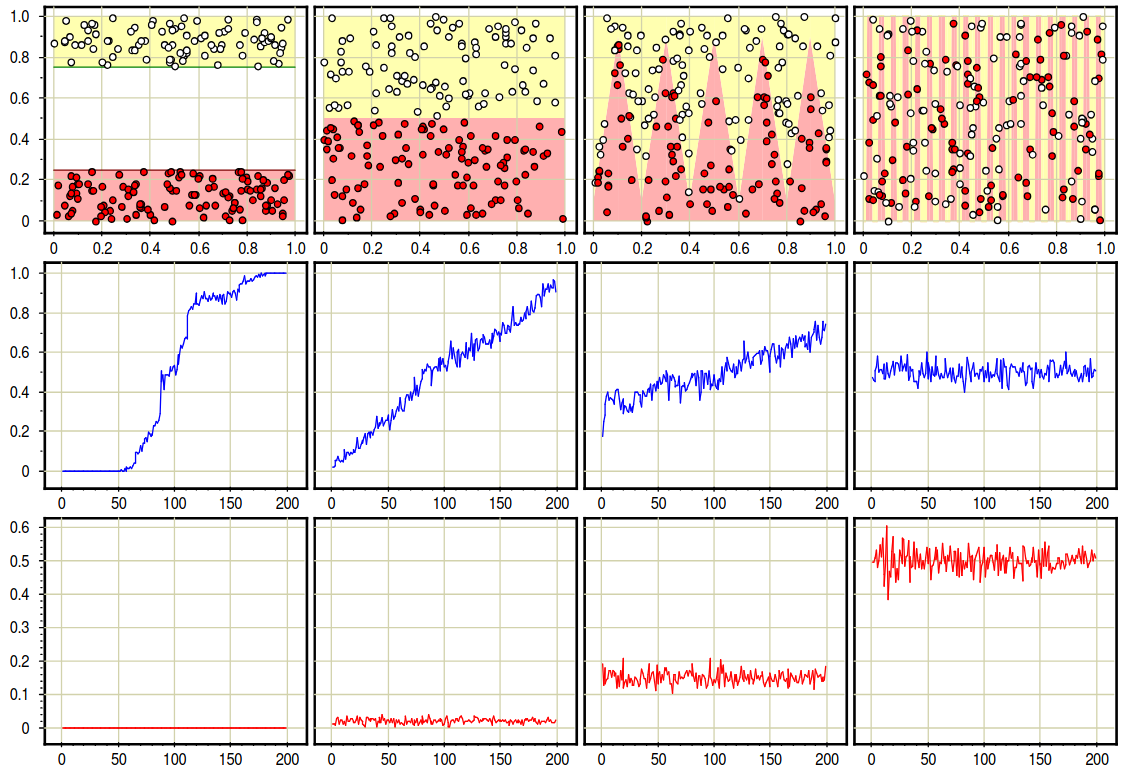
\includegraphics[width=\textwidth]{chapters/metric/images/compact.png}
	\label{fig:compact}
	\caption{
		Верхний ряд - два класса, средний ряд - профиль компактности $\Pi(m)$, нижний ряд - зависимость CCV от длины контроля.
	}
\end{figure}

\noindent
\textbf{Первый набор}: классы разнесены далеко друг от друга. Из профиля компактности видно, что у всех объектов 50 ближайших соседей лежат в своем классе. Значит, у этой задачи будет почти 100\% качество при использовании kNN алгоритма. \\

\noindent
\textbf{Второй набор}: классы расположены так, что между ними проходит граница. Профиль компактности линейно растет при увеличении числа соседей, причем для малого количества соседей имеем ненулевой $\Pi(m)$. \\

\noindent
\textbf{Третий набор}: классы проникают друг в друга. Начальный участок профиля компактности выше нуля, значит, у алгоритма kNN будет больше ошибок. \\

\noindent
\textbf{Четвертый набор}: классы равномерно распределены. Профиль компактности находится на уровне $0.5$, и у kNN нет возможности адекватно решить данную задачу: имеем случайное гадание. \\

\noindent
\textbf{Замечание}: из нижнего ряда имеем, что CCV почти не зависит от длины контроля, то есть нет причины выделять в контрольную выборку более одного объекта и достаточно использовать CCV(1).



\subsection{Задачи}

\noindent
\textbf{Задача 1}: доказать точное выражение CCV для метода 1NN.

\noindent
\textbf{Решение}:

\begin{equation*}
	\begin{gathered} \operatorname{CCV}=\frac{1}{C_L^{\ell}} \sum_{X^{\ell} \sqcup X^k} \frac{1}{k} \sum_{i=1}^L\left[x_i \in X^k\right]\left[a\left(x_i ; X^{\ell}\right) \neq y_i\right]= \\ =\sum_{X^{\ell} \sqcup X^k} \sum_{i=1}^L \sum_{m=1}^k \frac{\left[y_i^{(m)} \neq y_i\right]}{k C_L^{\ell}}\left[x_i^{(m)} \in X^{\ell}\right]\left[x_i, x_i^{(1)}, \ldots, x_i^{(m-1)} \in X^k\right]= \\ =\sum_{m=1}^k \sum_{i=1}^L \frac{\left[y_i^{(m)} \neq y_i\right]}{k C_L^{\ell}} \sum_{X^{\ell} \sqcup X^k}\left[x_i^{(m)} \in X^{\ell}\right]\left[x_i, x_i^{(1)}, \ldots, x_i^{(m-1)} \in X^k\right]= \\ =\sum_{m=1}^k \sum_{i=1}^L \frac{\left[y_i^{(m)} \neq y_i\right]}{k C_L^{\ell}} C_{L-1-m}^{\ell-1}=\sum_{m=1}^k \underbrace{\frac{1}{\sum_{i=1}^L\left[y_i^{(m)} \neq y_i\right]} \frac{C_{L-1-m}^{\ell-1}}{C_{L-1}^{\ell}} .}_{\Pi(m)} 
	\end{gathered}
\end{equation*}

\noindent
\textbf{Задача 2}: получить выражения для CCV при малой длине контроля.

\noindent
\textbf{Решение}:

\begin{equation*}
	\begin{aligned} 
		\mathrm{CCV(1)}=\Pi(1)=\mathrm{LOO}
	\end{aligned}
\end{equation*}

\begin{equation*}
	\begin{aligned} 
		\mathrm{CCV(2)}=\Pi(1) \frac{\ell}{\ell+1}+\Pi(2) \frac{1}{\ell+1}
	\end{aligned}
\end{equation*}

\begin{equation*}
	\begin{aligned}
		\mathrm{CCV(3)}=\Pi(1) \frac{\ell}{\ell+2}+\Pi(2) \frac{2 \ell}{(\ell+1)(\ell+2)}+\Pi(3) \frac{2}{(\ell+1)(\ell+2)} 
	\end{aligned}
\end{equation*}

\noindent
При достаточно гладком распределении $\Pi(m)$ CCV слабо зависит от длины контроля.  \\ \\

\noindent
\textbf{Задача 3}: получить скорость спада множителя при $\Pi(m)$ в выражении для CCV.

\noindent
\textbf{Решение}:

\begin{equation*}
	R(m)=\frac{C_{L-1-m}^{\ell-1}}{C_{L-1}^{\ell}};
\end{equation*}

\begin{equation*}
	\frac{R(m+1)}{R(m)}=1-\frac{\ell-1}{L-1-m}<\frac{k}{L-1} .
\end{equation*}

\noindent
То есть $R(m)$ стремится к нулю быстрее геометрической прогрессии.


\subsection{Минимизация CСV}

Из рассмотренных графиков и приведенных задач получили, что 
$\mathrm{CCV}$ тем меньше, чем чаще близкие объекты лежат в одном классе. Значит, минимизируя CСV, можно добиться лучшего результата работы алгоритма k ближайших соседей. CCV почти не зависит от длины контроля для kNN, поэтому достаточно использовать CCV(1) равный LOO.


\section*{Приближенные методы поиска ближайщих соседей (ANN)}

Иногда методы точного поиска ближайших соседей могут быть достаточно времязатратными и вычислительно сложными. Но зачастую реальные задачи не требуют вычислять именно самых близких соседей, и достаточно найти всего несколько наиболее близких. Для этой цели нам подойдут приближенные методы поиска, рассмотренные ниже.

\subsection{Random projection trees - \textbf{Annoy}}

Ряд алгоритмов приближенного поиска основан на деревьях, которые часто применяются для поиска соседей. Одним из наиболее известных и зарекомендовавших себя методов из данного семейства является алгорим \textbf{Annoy}. Опишем принцип его работы.

Пусть у нас есть обучающая выборка. Наша цель — построить структуру данных, которая позволит нам находить ближайшие точки к любой точке запроса. Для начала выберем из нее два объекта случайным образом. Между ними симметрично проводится разделяющая гиперплоскость. Далее в каждом из полученных полупространств снова выбирается два случайных элемента из набора данных, и уже между ними проводятся разделяющие гиперплоскости.

\begin{figure}[ht]
    \centering
    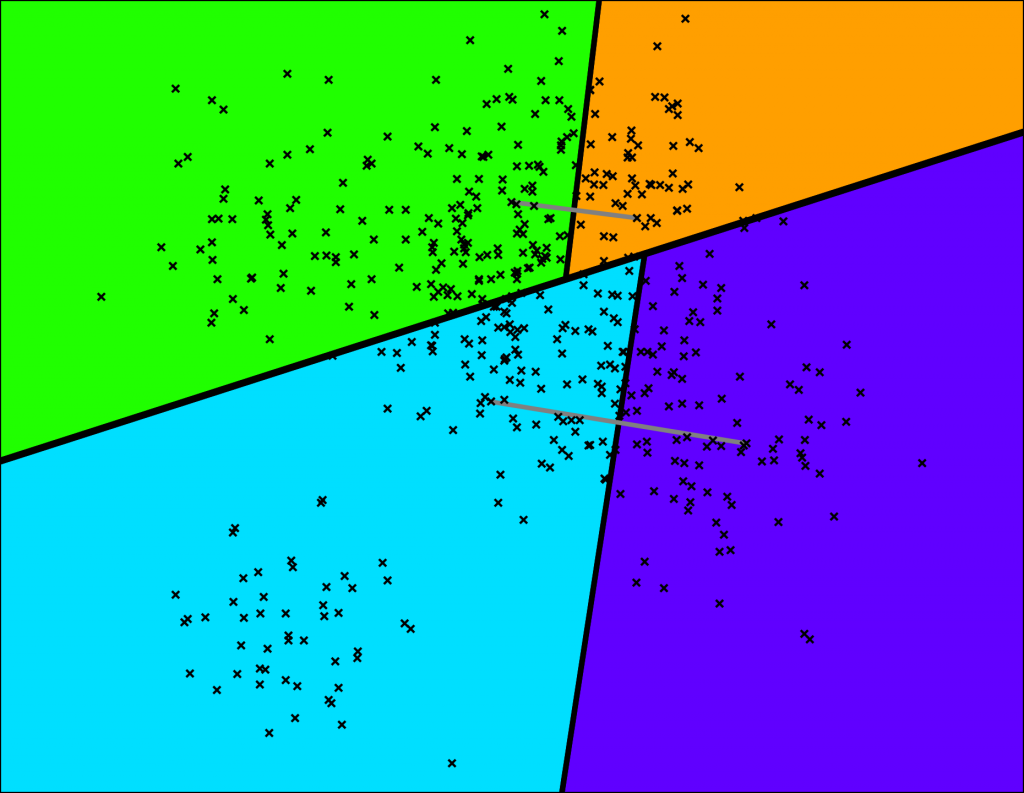
\includegraphics[width=\textwidth]{chapters/metric/images/tree-2.png}
    \caption{Разделение пространства гиперплоскостями в алгоритме Annoy.}
    \label{fig:annoy}
\end{figure}

Данная процедура продолжается итеративно, пока в каждой области останется не более $K$ объектов. Здесь $K$ является подбираемым гиперпараметром. На самомо деле, данная процедура чем-то похожа на то, как работают k-d-деревья.

\begin{figure}[ht]
    \centering
    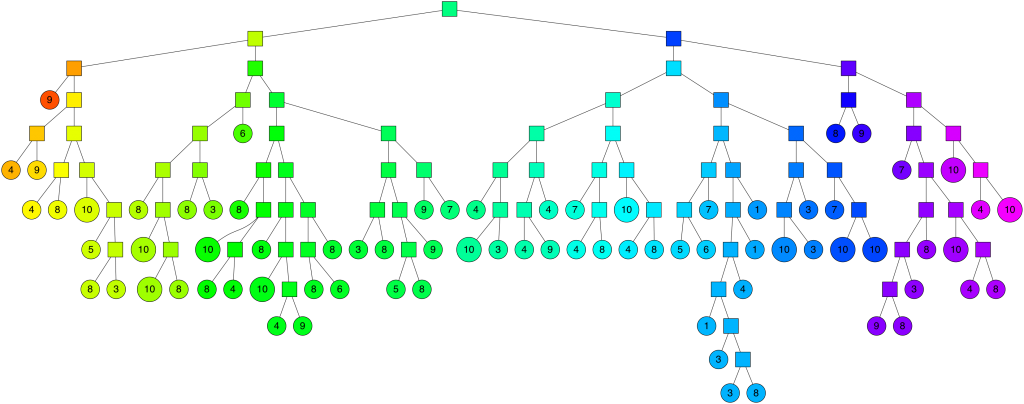
\includegraphics[width=\textwidth]{chapters/metric/images/tree-full.png}
    \caption{В результате работы алгоритма получаем бинарное дерево.}
    \label{fig:full-tree}
\end{figure}

В результате работы вышеописанного алгоритма мы получим бинарное дерево (рис. 3) (глубина порядка $O(logN)$), спускаясь по которому, найдем область с целевым объектом и нектоторым количеством близких к нему элементов. Давайте попробуем найти точку, обозначенную красным крестом на рис. 4.

\begin{figure}[ht]
    \centering
    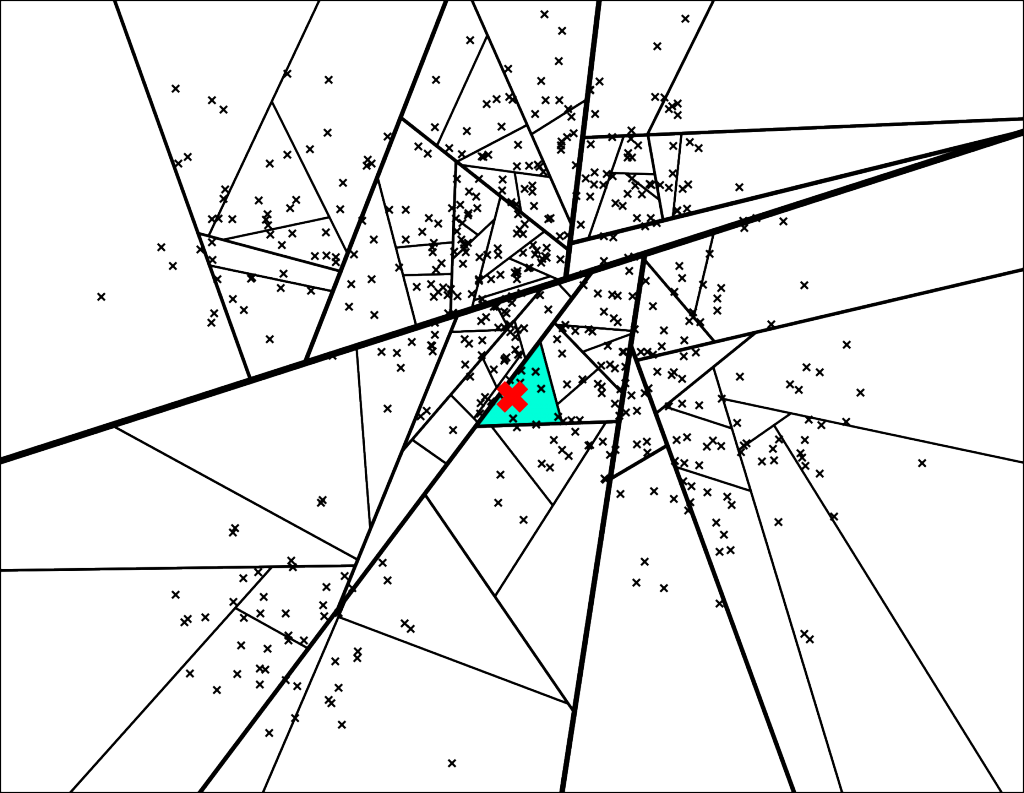
\includegraphics[width=\textwidth]{chapters/metric/images/heap-pos.png}
    \caption{Поиск для точки, обозначенной красным крестом.}
    \label{fig:heap-pos}
\end{figure}

То, как будет выглядеть путь вниз по бинарному дереву в данном случае, показано на рис. 5. 

\begin{figure}[ht]
    \centering
    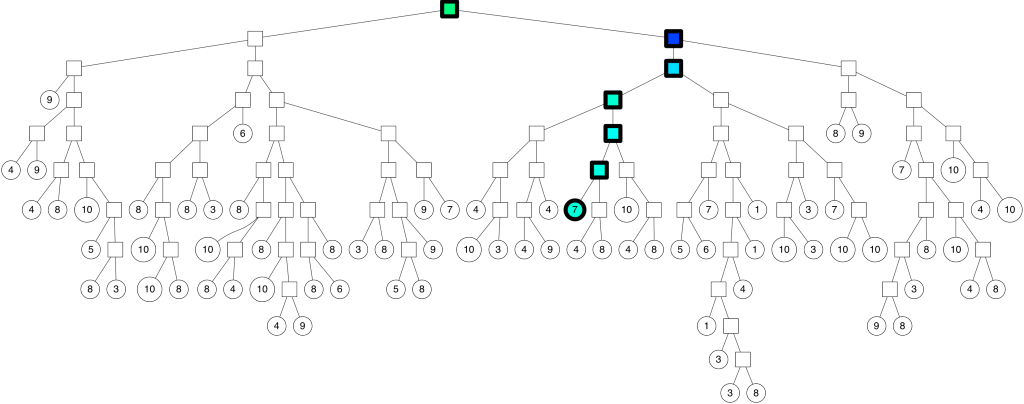
\includegraphics[width=\textwidth]{chapters/metric/images/heap-pos-graphviz.png}
    \caption{Поиск точки.}
    \label{fig:heap-pos-graph}
\end{figure}

Таким образом, мы получаем 7 ближайших соседей. Уже хороший результат, но достаточно ли нам этого?

\textbf{Задача 1}

Мы проделали весь алгоритм, описанный выше, и получили для некторой точки 7 ближайших соседей. На самом деле, нам этого недостаточно, попробуйте подумать, почему. 

\textbf{Решение}. Во-первых, может произойти ситуация, что нам нужно не 7 ближайших соседей, а больше.  Например, методы приближенного поиска соседей используются для подбора рекомендаций фильмов, и в такой задаче нам необходимо найти около 10-15 наиболее похожих картин для пользователя. 
Во-вторых, некоторые из ближайших соседей на самом деле могут не попасть в итоговую область пространства и остаться за его пределами. 

Необходимо увеличить точность алгоритма при помощи составления леса из таких деревьев. Мы можем выполнить поиск по всем деревьям одновременно, и взять объединение соответствующих целевому объекту областей. Именно так работает алгоритм Annoy. 

\textbf{Задача 2}

Давайте подумаем, почему же методы приближенного поиска (ANN - approximate nearest neighbor) дают выйгрыш по времени и являются менее ресурсозатратными по сравнению с точными методами?

\textbf{Решение}. Если объем анализируемых данных становится слишком большим, что нередко встречается в рельаной жизни, то точные методы поиска ближайших соседей будут просматривать всю выборку данных, что займет огромное количество времени. А алгоритмы ANN не просматривают все объекты из датасета, следовательно, являются более быстрыми и эффективными. ANN — это алгоритм, который находит точку данных в наборе данных, которая очень близка к заданной точке запроса, но не обязательно является абсолютно ближайшей. Алгоритм точного поиска выполняет исчерпывающий поиск по всем данным, чтобы найти идеальное совпадение, тогда как алгоритм ANN остановится на совпадении, которое достаточно близко.

\textbf{Задача 3}

Оцените время построения модели Annoy для базы данных из 500 объектов.

\textbf{Решение}. Время поиска ближайших соседей для одного запроса в модели Annoy — $O(logN)$, где N — количество объектов в базе данных. А dремя построения модели Annoy для базы данных из 500 объектов составляет $O(N\cdot logN)$. Для $N = 500$ будет :

\[
    T = O(500 \cdot log500) 
\]
\[
    log500 \approx 2.7 
\]
\[
    T = O(500 \cdot 2.7) = O(1350)
\]

То есть время, необходимое для построения модели Annoy для 500 объектов, будет порядка 1350 операций.

\section{Отбор эталонных объектов}
Обучающие объекты делятся на три категории: эталоны (типичные представители классов), неинформативные (окружены объектами того же класса) и шумовые выбросы (расположены среди объектов чужого класса). Исключение шумовых и неинформативных объектов позволяет улучшить классификацию, сократить объём данных и ускорить поиск ближайших эталонов.

Алгоритм STOLP реализует эту идею, основываясь на весовой функции \( w(i, u) \). Он строит метрический алгоритм \( a(u; \Omega) \), где \( \Omega \subset X_\ell \) — множество эталонов. 

Отступ объекта \( x_i \) относительно алгоритма \( a(x_i; \Omega) \), обозначенный как \( M(x_i, \Omega) \), используется для классификации объектов:
\begin{itemize}
    \item \( M(x_i, \Omega) < 0 \) — объект окружён чужими классами и считается выбросом;
    \item \( M(x_i, \Omega) > 0 \) — объект окружён своими классами и является либо эталоном, либо неинформативным.
\end{itemize}

\section{Компактность и профиль компактности}

\textbf{Определение 1.} Профиль компактности относительно множества эталонов \( \Omega \subseteq X^L \) определяется как:
\[
\Pi(m, \Omega) = \frac{1}{L} \sum_{i=1}^L \left[ y_i^{(m|\Omega)} \neq y_i \right],
\]
где \( x_i^{(m|\Omega)} \) — \( m \)-й сосед объекта \( x_i \) из множества \( \Omega \), а \( y_i \) — истинная метка класса объекта \( x_i \).


\textbf{Теорема 1.} Компактность множества эталонов \( \Omega \) вычисляется как:
\[
CCV(\Omega) = \frac{1}{L} \sum_{i=1}^L \sum_{m=1}^k \left[ y_i^{(m|\Omega)} \neq y_i \right] \cdot \frac{C_{L-1}^{L-1-m}}{C_L^{L-1}},
\]
где \( T(x_i, \Omega) \) — вклад объекта \( x_i \) в \( CCV \).


\subsection*{Жадный отбор эталонов по критерию $CCV(\Omega) \to \min$}

\textbf{Жадная стратегия удаления не-эталонов:}
\begin{enumerate}
    \item Инициализация: $\Omega := X^L$.
    \item Повторять:
    \begin{enumerate}
        \item Найти $x \in \Omega$, при котором $CCV(\Omega \setminus \{x\}) \to \min$.
        \item Удалить $x$: $\Omega := \Omega \setminus \{x\}$.
        \item Обновить $T(x_i, \Omega)$ для всех $x_i$, где $x \in kNN(x_i)$.
    \end{enumerate}
    пока $CCV$ уменьшается или практически не увеличивается.
\end{enumerate}

\textbf{Жадная стратегия добавления эталонов:}
\begin{enumerate}
    \item Инициализация: $\Omega := \{\text{по одному объекту от каждого класса}\}$.
    \item Повторять:
    \begin{enumerate}
        \item Найти $x \in X^L \setminus \Omega$, при котором $CCV(\Omega \cup \{x\}) \to \min$.
        \item Добавить $x$: $\Omega := \Omega \cup \{x\}$.
        \item Обновить $T(x_i, \Omega)$ для всех $x_i$, где $x \in kNN(x_i)$.
    \end{enumerate}
    пока $CCV$ уменьшается.
\end{enumerate}

\subsection*{Алгоритм: Отбор эталонных объектов STOLP}
\textbf{Вход:} 
\begin{itemize}
    \item \( X_\ell \) — обучающая выборка;
    \item \( \delta \) — порог фильтрации выбросов;
    \item \( \ell_0 \) — допустимая доля ошибок.
\end{itemize}
\textbf{Выход:}
\begin{itemize}
    \item Множество опорных объектов \( \Omega \subset X_\ell \).
\end{itemize}

\textbf{Алгоритм:}
\begin{enumerate}
    \item Для всех \( x_i \in X_\ell \) проверить, является ли \( x_i \) выбросом:
    \[
    \text{если } M(x_i, X_\ell) < \delta, \text{ то } X_{\ell-1} := X_\ell \setminus \{x_i\}; \quad \ell := \ell - 1;
    \]
    \item Инициализация: взять по одному эталону от каждого класса:
    \[
    \Omega := \arg \max_{x_i \in X_\ell, y \in Y} M(x_i, X_\ell);
    \]
    \item Пока \( \Omega \neq X_\ell \):
    \begin{itemize}
        \item Выделить множество объектов, на которых алгоритм \( a(u; \Omega) \) ошибается:
        \[
        E := \{x_i \in X_\ell \setminus \Omega : M(x_i, \Omega) < 0\};
        \]
        \item Если \( |E| < \ell_0 \), то выход.
        \item Присоединить к \( \Omega \) объект с наименьшим отступом:
        \[
        x_i := \arg \min_{x \in E} M(x, \Omega); \quad \Omega := \Omega \cup \{x_i\};
        \]
    \end{itemize}
\end{enumerate}



\subsection*{Результаты работы алгоритма}
Алгоритм делит обучающие объекты на три категории:
\begin{itemize}
    \item Шумовые выбросы, которые удаляются.
    \item Эталонные объекты, которые формируют подмножество $\Omega$.
    \item Неинформативные объекты, которые также удаляются.
\end{itemize}

Если гипотеза компактности верна, то большая часть обучающих объектов окажется неинформативной и будет отброшена, обеспечивая сжатие данных.

\subsection*{Оценка эффективности алгоритма STOLP}
Алгоритм STOLP имеет относительно низкую эффективность: добавление каждого эталона требует перебора объектов \( X_\ell \setminus \Omega \) и вычисления отступов относительно \( \Omega \), что приводит к сложности \( O(|\Omega|^2 \ell) \). Для ускорения можно добавлять несколько эталонов одновременно, выбирая их на большом расстоянии друг от друга, чтобы минимизировать влияние на отступы.

На этапе отсева выбросов допустимо вычислить отступы один раз и отбросить объекты с \( M(x_i, \Omega) < \delta \). Эффективная реализация включает процедуру обновления отступов \( M_i = M(x_i, \Omega) \), что позволяет гибко управлять вычислениями.

\subsection*{Задачи}

\textbf{Задача 1}
Докажите, что при использовании алгоритма STOLP отступ объекта \(M(x_i, \Omega)\) не зависит от порядка перебора эталонных объектов в \( \Omega \).

\textbf{Решение.}  
Рассмотрим отступ объекта \(x_i\) относительно множества эталонов \( \Omega \):
\[
M(x_i, \Omega) = \sum_{x_j \in \Omega} y_j w(\rho(x_i, x_j)).
\]
Порядок перебора объектов \(x_j \in \Omega\) не влияет на результат вычисления, так как операция суммирования коммутативна:
\[
\sum_{x_j \in \Omega} y_j w(\rho(x_i, x_j)) = \sum_{x_j \in \text{перестановке } \Omega} y_j w(\rho(x_i, x_j)).
\]
Таким образом, \(M(x_i, \Omega)\) остается неизменным независимо от порядка объектов в \( \Omega \). Это доказывает инвариантность отступа относительно перестановки эталонов.

\textbf{Задача 2}
В выборке \(X_\ell\) используется алгоритм STOLP для классификации объектов по двум классам. Выбросы имеют отступы \(M(x_i, \Omega) < \delta\), где \(\delta = 0\). Рассмотрим набор из трёх объектов:  
\begin{itemize}
    \item \(x_1: M(x_1, \Omega) = -0.5\),  
    \item \(x_2: M(x_2, \Omega) = 0.8\),  
    \item \(x_3: M(x_3, \Omega) = -0.2\).
\end{itemize}  
Определите, какие объекты будут исключены из обучающей выборки \(X_\ell\) на первом этапе алгоритма STOLP.

\textbf{Решение.}  
На этапе отсева выбросов STOLP удаляет объекты, для которых отступ \(M(x_i, \Omega) < \delta\). Учитывая \(\delta = 0\), удаляются объекты с отрицательными отступами.  

Проверяем отступы:  
\begin{itemize}
    \item \(M(x_1, \Omega) = -0.5 < 0\): \(x_1\) будет удалён,  
    \item \(M(x_2, \Omega) = 0.8 > 0\): \(x_2\) останется в выборке,  
    \item \(M(x_3, \Omega) = -0.2 < 0\): \(x_3\) будет удалён.  
\end{itemize}

\textbf{Ответ:} из обучающей выборки будут удалены объекты \(x_1\) и \(x_3\).

\textbf{Задача 3}
Докажите, что алгоритм STOLP допускает использование любых метрических функций \( \rho(x, x') \), если они удовлетворяют свойствам метрики.

\textbf{Решение.}  
Метрическая функция \( \rho(x, x') \) используется для вычисления отступов \(M(x_i, \Omega)\) и определяется через весовую функцию \(w(\rho)\). Для корректной работы алгоритма требуется, чтобы \( \rho(x, x') \) удовлетворяла следующим свойствам метрики:
\begin{enumerate}
    \item \textbf{Неотрицательность:} \(\rho(x, x') \geq 0\),  
    \item \textbf{Равенство нулю только при совпадении точек:} \(\rho(x, x') = 0 \iff x = x'\),  
    \item \textbf{Симметричность:} \(\rho(x, x') = \rho(x', x)\),  
    \item \textbf{Неравенство треугольника:} \(\rho(x, z) \leq \rho(x, y) + \rho(y, z)\).  
\end{enumerate}

Эти свойства гарантируют, что отступы \(M(x_i, \Omega)\) корректно отражают относительное положение объекта \(x_i\) относительно эталонов.  

Кроме того, функция \(w(\rho)\) должна быть убывающей, чтобы больший вклад в отступ вносили ближайшие эталоны, что не зависит от конкретной метрики, а лишь от её свойств.

\textbf{Вывод:} любой выбор функции \( \rho(x, x') \), удовлетворяющей свойствам метрики, допустим в алгоритме STOLP.

\section{Метод окна Парзена.}

Напомним идею метрического классификатора. Будем обозначать $x = (x^1, ..., x^n)$ - вектор признаков объекта $x$, $x_i = (x_i^1, ..., x_i^n)$ - вектор признаков объекта $x_i$. Пусть на пространстве признаков задана метрика $\rho$. Для произвольного объекта $x$ отранжируем объекты обучающей выборки $x_1, x_2, ..., x_l$:
\begin{equation*}
	\rho(x, x^{(1)}) \le \rho(x, x^{(2)}) \le ... \le \rho(x, x^{(l)}).
\end{equation*}
Таким образом, $x^{(i)}$ - $i-$й ближайший сосед объекта $x$ среди обучающий выборки, обозначим через $y^{(i)}$ ответ на нём. 

Метрический классификатор предлагает следующую модель зависимости:
\begin{equation*}
	\displaystyle a(x; X^l) = \arg\max_{y\in Y} \sum\limits_{i=1}^l[y^{(i)}=y]w(i,x), 
\end{equation*}
где $w(i,x)$ - некоторый вес, отражающий степень близости к объекту $x$ его $i-$го соседа. Вес неотрицателен и не возрастает по $i$. 

Кроме того, введём обозначение:
\begin{equation*}
	\displaystyle \Gamma_y(x) = \sum\limits_{i=1}^l[y^{(i)}=y]w(i,x) - \text{оценка близости объекта $x$ к классу $y$}. 
\end{equation*}

Напомним также, что метод $k$ ближайших соседей заключается в выборе в качестве весовой функции $w(i,x) = [i\le k]$. Среди недостатков этого метода выделим следующие:
\begin{itemize}
	\item в силу того, что функция близости дискретнозначная (принимает не более $k$ значений), часто попадаем в ситуацию неоднозначности классификации, когда $\Gamma_y(x) = \Gamma_z(x)$, $y\ne z$;
	\item метод не учитвает значение расстояний от объекта до ближайших соседей. Естественным кажется использование меньшего веса для далёкого объекта, даже если он попадаёт в $k$ ближайших.
\end{itemize}

Для борьбы с этими недостатков модифицируем веса следующим образом:
\begin{equation*}
	w(i,x) = [i\le k]w_i, \text{где $w_i$ зависит только от номера соседа}.
\end{equation*}

Тем самым, получим метод $k$ взвешенных ближайших соседей. В качестве $w_i$ можно брать, например, линейно убывающие веса $\displaystyle w_i = \frac{k+1-i}{k}$ или экспоненциально убывающие веса $w_i = q^i$, $0 < q < 1$.

Однако линейно убывающие веса всё ещё допускают неоднозначность классификации. Кроме того, метод по-прежнему не учитывает расстояния между объектами. 

Наконец, положим
\begin{equation*}
	\displaystyle w(i,x) = K\left(\frac{\rho(x, x^{(i)})}{h}\right),
\end{equation*}
где $K(r)$ - невозрастающая функция, определённая на неотрицательных числах, называемая ядром, положительная на отркезке $[0,1]$ и равная нулю вне его, $h$ - ширина окна. 

Таким образом, получим метод окна Парзена фиксированной ширины:
\begin{equation*}
	\displaystyle a(x; X^l, h, K) = \arg\max_{y\in Y} \sum\limits_{i=1}^l[y^{(i)}=y]K\left(\frac{\rho(x, x^{(i)})}{h}\right). 
\end{equation*}

Мы видим, что такой метод для каждого объекта $x$ рассматривает только объекты обучающей выборки, находящиеся на расстоянии не больше $h$ от $x$. Причём, чем дальше объект от $x$, тем  меньший вклад он даёт в оценку близости.

\textit{Замечание.} Вообще говоря, в качестве ядра можно брать функции, которые принимают ненулевые значения вне отрезка $[0,1]$, однако тогда они подбираются быстро убывающими (см. далее гауссовское ядро).

Заметим, что если расстояние от объекта $x$ до всех объектов обучающей выборки больше $h$, то построенный метод не может классифицировать $x$, так как в таком случае $\displaystyle\sum\limits_{i=1}^l[y^{(i)}=y]K\left(\frac{\rho(x, x^{(i)})}{h}\right) \equiv 0$. Это соображение наталкивает на использование метода окна Парзена переменной ширины:

\begin{equation*}
	\displaystyle a(x; X^l, h, K) = \arg\max_{y\in Y} \sum\limits_{i=1}^l[y^{(i)}=y]K\left(\frac{\rho(x, x^{(i)})}{\rho(x, x^{(k+1)})}\right). 
\end{equation*}

\textit{Замечание.} В знаменателе в ядре стоит расстояние до $k+1-$го соседа, так как на практике зачастую берутся ядра, которые в точке $1$ равны $0$. Таким образом, метод окна Парзена переменной ширины учитывает именно $k$ ближайших соседей объекта.

Для подбора наилучшей модели оптимизируются параматры:
\begin{itemize}
	\item ширина окна $h$ или количество сосеседей $k$;
	\item ядро $K$.
\end{itemize}

Выше мы считали, что ядро определено на неотрицательной полуоси. Эквивалентно, можно считать, что ядро определено на всей действительной оси, является чётной функцией, невозрастающей на отрезке $[0,1]$ (и, как правило, равна $0$ вне отрезка $[-1,1]$). В таком случае расстояние между объектами можно понимать как ориентированное. Однако, нетружно видеть, что ориентация ни на что не влияет. Приведём примеры наиболее часто используемых ядер:
\begin{itemize}
	\item $\displaystyle K_1(r) = \frac{3}{4}(1-r^2)[r\le1]$ - ядро Епанечникова;
	\item $\displaystyle K_2(r) = \frac{15}{16}(1-r^2)^2[r\le1]$ - квартическое ядро;
	\item $\displaystyle K_3(r) = (1-|r|)[r\le1]$ - треугольное ядро; 
	\item $\displaystyle K_4(r) = \frac{1}{2}[r\le1]$ - прямоугольное ядро; \item $\displaystyle K_5(r) = \frac{1}{\sqrt{2\pi}}e^{-r^2/2}$ - гауссовское ядро.
\end{itemize}
Числовые коэффициенты выбираются из соображений нормировки: $\displaystyle\int\limits_{-\infty}^{+\infty} K_i(r)dr = 1$.

\textbf{Задача 1.} Докажите, что метод окна Парзена фиксированной ширины можно переписать следующим образом:

\begin{equation*}
	\displaystyle a(x; X^l, h, K) = \arg\max_{y\in Y} \sum\limits_{i=1}^l[y_i=y]K\left(\frac{\rho(x, x_i)}{h}\right),
\end{equation*}
т.е. объекты обучающей выборки не обязательно ранжировать по расстоянию до объекта.

\textbf{Доказательство.} Заметим, что при любом фиксированном $y\in Y$ справедливо равенство $\displaystyle\sum\limits_{i=1}^l[y_i=y]K\left(\frac{\rho(x, x_i)}{h}\right) = \sum\limits_{i=1}^l[y^{(i)}=y]K\left(\frac{\rho(x, x^{(i)})}{h}\right)$, поскольку каждый объект обучающей выборки в обеих суммах участвует лишь единожды и значение соответствующего слагаемого не зависит от номера объекта. Отметим, что метод окна Парзена переменной ширины также можно переписать аналогичным образом.
\\

\textbf{Задача 2.} Вася решает методом окна Парзена фиксированной ширины задачу классификации объектов на $8$ классов по $3$ вещественным признакам. Все признаки объектов в обучающей выборке принимают значения, по модулю не меньшие $1$, и объекты $i-$го класса попадают в $i-$й октант пространства признаков. Вася использует евклидову метрику на пространстве признаков и берёт ширину окна $h = 1$. К какому из классов может его классификатор отнести точку $0$?

\textbf{Ответ.} Ни к какому.

\textbf{Решение.} По условию расстояние между $0$ и объектом обучающей выборки $\rho(x_i,0)\ge\sqrt{(1-0)^2+(1-0)^2+(1-0)^2} = \sqrt{3} > 1 = h$. Таким образом, ни одна точка обучающей выобрки не попадает в нужное окно с центром в нуле.

\textbf{Задача 3.} Докажите, что в качестве ядер в методе окна Парзена фиксированной ширины также можно брать выпуклую комбинацию ядер $K_1$, $K_2$, $K_3$, $K_4$ из примеров выше.

\textbf{Доказательство.} Заметим, что выпуклая комбинация также будет положительна при $|r|\le 1$ и нулевая вне этого отрезка, чётна и не убывает на отрезке $[0,1]$. Более того, также сохраняется нормировка: 
\begin{equation*}
	\displaystyle\int\limits_{-1}^{1}\left[\alpha_1K_1(r)+\alpha_2K_2(r) +\alpha_3K_3(r)+\alpha_4K_4(r)\right]dr = \alpha_1 + \alpha_2 +\alpha_3 +\alpha_4 =1.
\end{equation*}

\section{Метод потенциальных функций}

Метод потенциальных функций - метрический классификатор, частный случай метода ближайших соседей. Позволяет с помощью простого алгоритма оценивать вес («важность») объектов обучающей выборки при решении задачи классификации.

В общем виде, алгоритм ближайших соседей есть:
\begin{equation*}
	\displaystyle a(x; X^l) = \arg\max_{y\in Y} \sum\limits_{i=1}^l[y^{(i)}=y]w(i,x), 
\end{equation*}

где $w(i,x)$ — вес, степень близости к объекту $x$ его $i$-го соседа.

Метод потенциальных функций заключается в выборе в качестве веса $w(i,x)$, функции следующего вида:

\begin{equation*}
	\displaystyle w(i,x) = \gamma^{(i)} K\left(\frac{\rho(x, x^{(i)})}{h^{(i)}}\right),
\end{equation*}

где:

\begin{itemize}
	\item $K(r)$ -- ядро, не возрастает и положительно на $[0, 1]$,
	\item $\gamma^{(i)} \ge 0$ -- <<заряд>> объекта $x^{(i)}$, 
	\item $h^{(i)} > 0$ -- параметр, задающий <<ширину потенциала>> объекта $x^{(i)}$. 
\end{itemize}

Основная идея метода была навеяна электростатическим взаимодействием элементарных частиц. Известно, что потенциал («мера воздействия») электрического поля элементарной заряженной частицы в некоторой точке пространства пропорционален отношению заряда частицы ($Q$) к расстоянию до частицы ($r$): $\varphi(r) \sim \frac{Q}{r}$. Из-за этого в качестве $K(r)$ часто выступают функции: $\frac{1}{r}$ или $\frac{1}{r+a}$.

Метод потенциальных функций реализует полную аналогию указанного выше примера. При классификации объект проверяется на близость к объектам из обучающей выборки. Считается, что объекты из обучающей выборки «заряжены» своим классом, а мера «важности» каждого из них при классификации зависит от его «заряда» и расстояния до классифицируемого объекта.

\subsection{Подбор параметров}

Отметим, что параметрическую модель зависимости метода потенциальных функций можно существенно упросить (см. задачу ниже):

\begin{equation*}
	\displaystyle a(x; X^l) = \arg\max_{y\in Y} \sum\limits_{i=1}^l[y_i=y]\gamma_i K\left(\frac{\rho(x, x_i)}{h_i}\right).
\end{equation*}

Из выражения выше следует, что в методе потенциальных функций используются две группы параметров: $\{h_i\}$ и $\{\gamma_i\}$.

«Ширина окна потенциала» $h_i$ выбирается для каждого объекта из эмпирических соображений. «Заряд» $\gamma_i$ объектов выборки можно подобрать, исходя из информации, содержащейся в выборке. Ниже приведен алгоритм, который позволяет «обучать» параметры $\gamma_1, \dots, \gamma_n$, то есть подбирать их значения по обучающей выборке $X^l$.

\subsection*{Алгоритм подбора параметров $\{\gamma_i\}$}

\noindent \textbf{Вход:} обучающая выборка из l пар «объект-ответ» -- $X^l=\left((x_1,y_1), \dots, (x_l,y_l) \right)$.

\noindent \textbf{Выход:} значения параметров $\gamma_i$ для всех $i=\overline{1,l}$.

\noindent \textbf{Описание:}

\begin{enumerate}
	\item  Инициализация: $\gamma_i:=0$ для всех $i=\overline{1,l}$; 
	\item Повторять пункты $3-4$, пока эмпирический риск $Q(a,X^l) > \varepsilon$ (то есть пока процесс не стабилизируется):  
	\item Выбрать очередной объект $x_i$ из выборки $X^l$;
	\item Если $a(x_i) \not= y_i$, то $\gamma_i:=\gamma_i+1$;
	\item Вернуть значения $\gamma_i$ для всех $i=\overline{1,l}$.
\end{enumerate}

\subsection{Преимущества и недостатки}

Преимущества метода потенциальных функций:

\begin{itemize}
	\item Метод прост для понимания и алгоритмической реализации;
	\item Порождает потоковый алгоритм; 
	\item Хранит лишь часть выборки, следовательно, экономит память.
\end{itemize}

\noindent Недостатки метода:

\begin{itemize}
	\item Порождаемый алгоритм медленно сходится;
	\item Параметры $\{\gamma_i\}$ и $\{h_i\}$ настраиваются слишком грубо; 
	\item Значения параметров $\gamma_1,\dots,\gamma_l$ зависят от порядка выбора объектов из выборки $X^l$.
\end{itemize}

\subsection{Задачи для самопроверки}

\subsection*{Задача 1.}
Покажите, что параметрическую модель зависимости метода потенциальных функций можно переписать в следующем виде:

\begin{equation*}
	\displaystyle a(x; X^l) = \arg\max_{y\in Y} \sum\limits_{i=1}^l[y_i=y]\gamma_i K\left(\frac{\rho(x, x_i)}{h_i}\right).
\end{equation*}

\subsection*{Решение.}

Ответ следует из независимости суммы от перестановки слагаемых. $\forall y \in Y$:
\begin{equation*}
	\displaystyle 
	\sum\limits_{i=1}^l[y^{(i)}=y]\gamma^{(i)} K\left(\frac{\rho(x, x^{(i)})}{h^{(i)}}\right)
	= \sum\limits_{i=1}^l[y_i=y]\gamma_i K\left(\frac{\rho(x, x_i)}{h_i}\right).
\end{equation*}


\subsection*{Задача 2.}

Покажите, что метод потенциальных функций можно свести к линейному классификатору в случае $Y=\{-1, +1\}$ (бинарная классификация).

\subsection*{Решение.}

Обозначим $\Gamma_y(x) = \sum\limits_{i=1}^l[y^{(i)}=y]w(i,x)$ - оценка близости объекта $x$ к классу $y$. Тогда получим:
\begin{equation*}
	\displaystyle a(x; X^l) = \arg\max_{y\in Y} \Gamma_y(x) = \text{sign} \left(\Gamma_{+1}(x) - \Gamma_{-1}(x)\right) =  \text{sign} \sum\limits_{i=1}^l \gamma_i y_i K\left(\frac{\rho(x, x_i)}{h_i}\right),
\end{equation*}

что совпадает с линейной моделью классификации 
\begin{equation*}
	\displaystyle a(x; X^l) = \text{sign} \sum\limits_{j=1}^n \gamma_j f_j(x),
\end{equation*}

где

\begin{itemize}
	\item $f_j(x) = y_j K\left(\frac{\rho(x, x_j)}{h_j}\right)$ -- новые признаки объекта x,
	\item $\gamma_j$ -- веса линейного классификатора, 
	\item $n = l$ -- число признаков равно числу объектов обучения.
\end{itemize}

\subsection*{Задача 3.}

Привести пример выборки $(x_1, y_1),\dots,(x_l, y_l)$, такой, что метод потенциальных функций построит модель с эмпирическим риском $ Q(a,X^l) = \frac{1}{l} \sum\limits_{i=1}^{l} [a(x_i) \neq y_i] = \frac{1}{l}$.

\subsection*{Решение.}

Рассмотрим $l$-мерное пространство признаков $X=R^l$. В качестве выборки можно взять набор объектов, геометрически находящихся в вершинах $l$-симплекса. Тогда $\rho(x_i, x_j) = \text{const}$ (для простоты положим $\rho(x_i, x_j) = 1$). Остается лишь определить множество ответов: $y_1=+1, y_2=+1, \dots, y_{l-1}=+1, y_l=-1$. Используя результат задачи 2 (положив $h_i=1$), получим:

\begin{equation*}
	\displaystyle a(x; X^l) =  \text{sign} ( \sum\limits_{i=1}^{l-1} \gamma_i - \gamma_l).
\end{equation*}

Алгоритм подбора параметров $\{\gamma_i\}$ приведет к следующему набору (уже на второй итерации): $\gamma_1=1, \dots, \gamma_{l-1}=0, \gamma_l=1$. Т.е. $\forall x \in X^l$ 
\begin{equation*}
	\displaystyle a(x; X^l) = 1.
\end{equation*}

Воспользовавшись формулой для эмпирического риска получаем требуемое.
